\chapter{The Multiple Cause Mixture Model}
\label{ch:MCMM}

\section{Introduction}
\label{sec:mcmm:intro}
Multimorph, as an unsupervised learning system, must be
driven by an unsupervised learning algorithm, a procedure that induces categories from raw, unlabeled data.
This chapter discusses Multimorph's core learning algorithm, the Multiple Cause Mixture Model (MCMM) \citep{saund:94} 

This chapter is a culmination of the chain of reasoning established in the preceding three chapters.
In chapters~\ref{ch:intro} and \ref{ch:lit-review}, we saw that it was precisely 
the set of \emph{nonlinear-nonsequential} models that were capable of representing 
nonconcatenative morphological structure, and moreover, that this capacity stems from the properties \emph{nonlinearity}
and \emph{nonsequentiality}. Furthermore, we saw in 
chapter~\ref{ch:graph} that bipartite graphs (or bipartite graphical algorithms) were a 
subset of NLNS algorithms. In fact, the bipartite structure of such graphs turns out to 
be a particularly coherent way to capture nonlinearity and nonsequentiality.
The present chapter homes in on a particular kind of bipartite learning algorithm, namely 
the MCMM. Thus, the present chapter, when taken in the context of the preceding chapters, 
explains the rationale and theoretical significance of my choosing an MCMM 
in particular to serve as Multimorph's learning algorithm.

This chapter is organized as follows: Section~\ref{sec:architecture} first lays out the key components 
of an MCMM's structure, i.e., the attributes that all MCMMs share. 
Section~\ref{sec:context} then proceeds to place MCMMs in a larger context of 
unsupervised learning algorithms, demonstrating 
the similarities and differences between MCMMs and other types of
 learning algorithms such as Restricted Boltzmann Machines (RBMs) \citep{smolensky:1986, hinton:2002}
 and Latent Dirichlet Allocation (LDA) \citep{blei-et-al:2003}. Section~\ref{sec:mixing-function} 
 focuses on a particularly important component of an MCMM, namely its 
 \emph{mixing function}, which is a type of activation function, that is, a 
 function that determines the activities of nodes in neural networks.  
Finally, section~\ref{sec:mcmm-learning} discusses the means by which 
MCMMs learn, paying particular attention to Multimorph's MCMM.

\section{Basic MCMM Architecture}
\label{sec:architecture}

In \citet{saund:94}, the term \emph{multiple cause mixture model} refers to a family of algorithms rather than to a single, 
specific algorithm. It does, however, denote a specific category of algorithm, and since
MCMMs constitute a definite category, 
all MCMMs share certain key attributes.
These attributes are 
%in large part 
the subject of this section. 

An MCMM is a graphical model consisting of two layers of nodes (or units): a \emph{surface} (or \emph{visible}) 
layer and a \emph{hidden} layer.
These two layers are illustrated in figure~\ref{fig:mcmm}, where $\mathbf{m}_i$ 
is the vector of hidden units, and $\mathbf{r}_i$ is the layer of surface units. The layer $\mathbf{r}_i$ is actually a  ``working'' reconstruction of the original surface-unit vector $\mathbf{x}_i$, but we will nonetheless refer to it as the surface layer, and its components (or nodes) as surface units.\footnote{Saund 
uses $\mathbf{d}$ 
rather than $\mathbf{x}$ to denote this vector. We use $\mathbf{x}$ because it seems to be more widely
used elsewhere to denote data points. We also use $\mathbf{d}$ to denote the \emph{direction vector} later in this chapter, so using $\mathbf{x}$ to denote data points helps to avoid confusion.}
As a working
reconstruction, $\mathbf{r}_i$ is dynamic; it evolves as the learning progresses and thus
becomes increasingly similar to $\mathbf{x}_i$. 

Notice in figure~\ref{fig:mcmm} that there are no connections between $\mathbf{x}_i$ and $\mathbf{r}_i$, nor between 
$\mathbf{x}_i$ and $\mathbf{m}_i$. The vector $\mathbf{x}_i$ is thus not an integrated component of the graphical 
model. Its role is merely to serve as a target for the reconstruction vector $\mathbf{r}_i$. 
The goal of the system as a learning model is therefore to get $\mathbf{r}_i$ to 
match $\mathbf{x}_i$, that is, to reconstruct the component values of $\mathbf{x}_i$ in 
the vector $\mathbf{r}_i$. The process that achieves this reconstruction is the learning process and is discussed in detail in section~\ref{sec:mcmm-learning}.

\begin{figure}[t]
\begin{mdframed}
%\begin{center}
\centering
\small
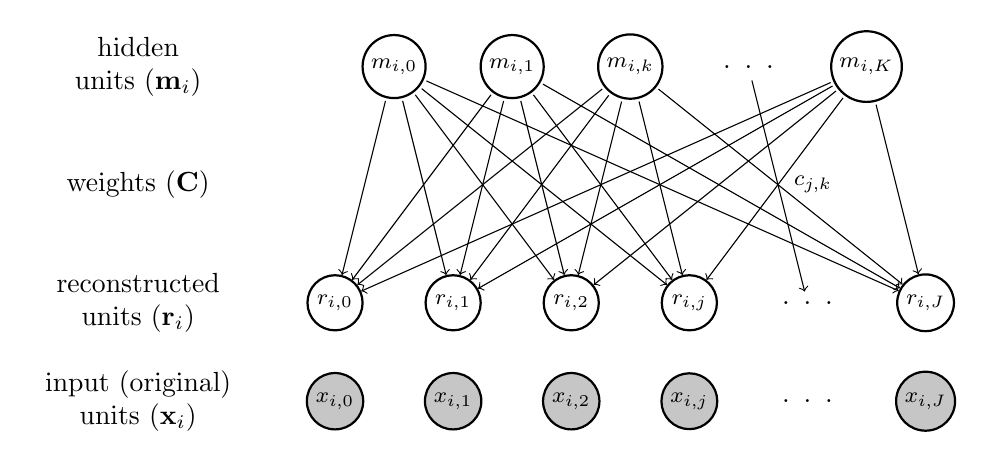
\begin{tikzpicture}[shorten <=1pt,->,draw=black!100]
	\def \rowtwoht{4.25cm}
	\def \weightlevel{2.75cm}
	\def \rowoneht{1.25cm}
	\def \basement{0cm}
	\tikzstyle{m-node}=[circle,draw=black!100,thick,inner sep=2pt,minimum size=7mm]
	\tikzstyle{r-node}=[circle,draw=black!100,thick,inner sep=2pt,minimum size=7mm]
	\tikzstyle{d-node}=[circle,draw=black!100,fill=gray!45,thick,inner sep=2pt,minimum size=7mm]
	\tikzstyle{dots}=[text width=5ex, text centered]
	\tikzstyle{annot}=[text width=17ex, text centered]
	% labels
	\node[annot] (hidden-layer) at (0cm,\rowtwoht) {hidden units ($\mathbf{m}_i$)};
	\node[annot] (weights) at (0cm,\weightlevel) {weights ($\mathbf{C}$)};
	\node[annot] (r-layer) at (0cm,\rowoneht) {reconstructed units ($\mathbf{r}_i$)};
	\node[annot] (d-layer) at (0cm,\basement) {input (original) units ($\mathbf{x}_i$)};
	
	\node[dots] 	(m3)	at (7.75cm,\rowtwoht)	 	{. . .};
	\node[dots] 	(r4) 	at (8.5cm,\rowoneht)   		{. . .};
	\node[dots] 	(d4) 	at (8.5cm,\basement)   		{. . .};
	
	\footnotesize
	% hidden layer
	\node[m-node] 	(m0)	at (3.25cm,\rowtwoht)		{$m_{i,0}$};
	\node[m-node] 	(m1)	at (4.75cm,\rowtwoht)		{$m_{i,1}$};
	\node[m-node] 	(m2)	at (6.25cm,\rowtwoht)	 	{$m_{i,k}$};
	\node[m-node] 	(m4)	at (9.25cm,\rowtwoht)	 	{$m_{i,K}$};
	
	% reconstructed vector
	\node[r-node] 	(r0)	at (2.5cm,\rowoneht)		{$r_{i,0}$};
	\node[r-node] 	(r1)	at (4cm,\rowoneht)		{$r_{i,1}$};
	\node[r-node] 	(r2)	at (5.5cm,\rowoneht)	 	{$r_{i,2}$};
	\node[r-node] 	(r3)	at (7cm,\rowoneht) 		{$r_{i,j}$};
	\node[r-node] 	(r5) 	at (10cm,\rowoneht)   		{$r_{i,J}$};
	%\node[r-node] 	(r6) 	at (9.75cm,\rowoneht)   	{$r_{i,J}$};
	
	% data vector
	\node[d-node] 	(d0)	at (2.5cm,\basement)		{$x_{i,0}$};
	\node[d-node] 	(d1)	at (4cm,\basement)		{$x_{i,1}$};
	\node[d-node] 	(d2)	at (5.5cm,\basement)	 	{$x_{i,2}$};
	\node[d-node] 	(d3)	at (7cm,\basement) 		{$x_{i,j}$};
	\node[d-node] 	(d5) 	at (10cm,\basement)   		{$x_{i,J}$};
	%\node[d-node] 	(d6) 	at (9.75cm,\basement)   	{$x_{i,J}$};
	
	\path 
		(m0)	edge	node	{}	(r0)
		(m0)	edge	node	{}	(r1)
		(m0)	edge	node	{}	(r2)
		(m0)	edge	node	{}	(r3)
		(m0)	edge	node	{}	(r5)
		
		(m1)	edge	node	{}	(r0)
		(m1)	edge	node	{}	(r1)
		(m1)	edge	node	{}	(r2)
		(m1)	edge	node	{}	(r3)
		(m1)	edge	node	{}	(r5)
		
		(m2)	edge	node	{}	(r0)
		(m2)	edge	node	{}	(r1)
		(m2)	edge	node	{}	(r2)
		(m2)	edge	node	{}	(r3)
		(m2)	edge	node	{}	(r5)
		(m3)	edge	node[right=1mm]	{$c_{j,k}$}	(r4)
		%	
		(m4)	edge	node	{}	(r0)
		(m4)	edge	node	{}	(r1)
		(m4)	edge	node	{}	(r2)
		(m4)	edge	node	{}	(r3)
		(m4)	edge	node	{}	(r5);
		
\end{tikzpicture}
%\end{center}
\caption{Architecture of a Multiple Cause Mixture Model (MCMM)} 
\label{fig:mcmm}
\vspace{12pt}
\end{mdframed}
\end{figure}

The vector $\mathbf{x}_i$ is the $i$th row in the 
input corpus, that is, the $I \times J$ input-data matrix $\textbf{X}$. Each 
row in $\textbf{X}$ is a data point, a feature-vector representation of a word. 
The $J$ columns in  $\textbf{X}$ each represent a particular feature.
The identical subscript on $\mathbf{x}_i$ 
and $\mathbf{r}_i$ means that these vectors correspond to the same data 
point, and thus ultimately the same word (namely, the $i$th word). Notice that the hidden 
layer $\textbf{m}_i$ bears this same index and is thus also tied to the $i$th word. In particular, it 
is the 
\emph{cluster-membership vector} of the $i$th word; that is, it is the $i$th row of 
the $I \times K$ matrix 
$\mathbf{M}$.  Each column in the $\mathbf{M}$ matrix corresponds to a cluster, and thus so does each component $m_{i,k}$ of a cluster-membership vector. In particular, the $k$th component in a given cluster-membership vector corresponds to the $k$th cluster. It indicates whether or not $i$th data point is a member of this cluster. 

\section{Relationship to Other Unsupervised\\Learning Frameworks}
\label{sec:context}

In this section, we relate multiple cause mixture models to other frameworks for unsupervised learning. 
Multiple cause mixture models simultaneously belong to two distinct unsupervised-learning contexts. 
On the one hand, they are neural networks, and more specifically, they are \emph{autoencoders}, which are neural networks that learn without supervision \citep{bourlard:1988, dayan-and-zemel:95}. %, phongthong:2016}.
On the other hand, the very name 
\emph{multiple cause mixture model} 
contains the term \emph{mixture model}, which itself refers to a large class of unsupervised learning models. 
This section is therefore divided into two subsections: First, section~\ref{sec:autoencoders} 
considers MCMMs as neural networks, i.e., as autoencoders, using neural-network terminology 
to relate them to other autoencoders, particularly the classical autoencoder and the restricted Boltzmann machine (RBM).  Section~\ref{sec:mixture-models} then 
considers MCMMs from a \emph{mixture-model} perspective, discussing their 
relationship to standard mixture models as well as \emph{mixed-membership} 
(or \emph{admixture}) models. 

\subsection{Autoencoders}
\label{sec:autoencoders}
\citet[][p. 2]{dayan-and-zemel:95} describe the MCMM as a ``form of autoencoder network.'' 
They mean \emph{autoencoder} in a general sense, as a term for a class that encompasses several subtypes.  
In this general sense, an \emph{autoencoder} is any unsupervised graphical algorithm that
learns a compressed encoding of its input data. 
An autoencoder learns by iteratively testing and revising its internal model, improving it slightly with each iteration. 
%\citep{rumelhart-et-al:1985, hinton:1987, hinton:1987trans, hinton-and-salak:2006}.
%The autoencoder tests the suitability of a working encoding through \emph{reconstruction}, i.e., by attempting to recover or reconstruct the original data from the working encoding.
%Thus, at the beginning of each iteration, the autoencoder has 
The internal model consists of the values of its weights along with 
the values in the hidden-unit vectors $\textbf{m}_i$. The values 
of the weights are universal, applying to the whole data set, while 
each hidden-unit vector $\textbf{m}_i$ is specific to the $i$th data point. 
An autoencoder's learning process consists of two
loops: an \emph{inner loop} that iterates over the data-point indices $i \in I$, 
visiting each individual data point in turn, and an \emph{outer loop} that repeats 
the inner loop as many times as necessary.
An autoencoder tests the fitness of its working model by attempting to reconstruct each input data 
point from its internal representation (or encoding) of the data point 
and then measuring the \emph{reconstruction error}, the discrepancy between the reconstructed and original data vectors.  
It then makes adjustments to the model so as to reduce this error. % \citep{hinton:1987, hinton:1987trans}.

\begin{figure}[t]
\begin{mdframed}
%%\begin{minipage}{.3\textwidth}
\centering
\small
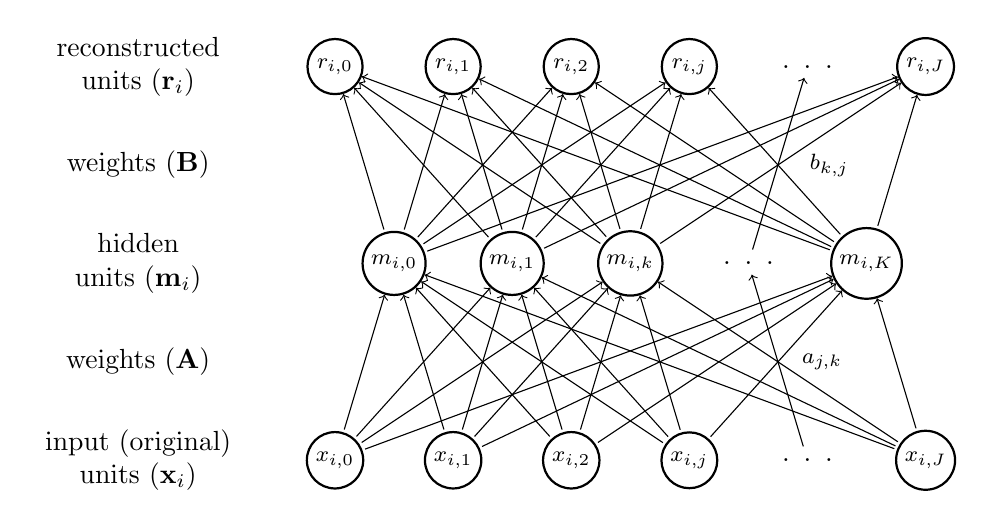
\begin{tikzpicture}[shorten <=1pt,->,draw=black!100]
	\def \rowtwoht{5cm}
	\def \weightstwo{3.75cm}
	\def \rowoneht{2.5cm}
	\def \weightsone{1.25cm}
	\def \basement{0cm}
	\tikzstyle{m-node}=[circle,draw=black!100,thick,inner sep=2pt,minimum size=7mm]
	\tikzstyle{r-node}=[circle,draw=black!100,thick,inner sep=2pt,minimum size=7mm]
	\tikzstyle{d-node}=[circle,draw=black!100,thick,inner sep=2pt,minimum size=7mm]
	\tikzstyle{dots}=[text width=5ex, text centered]
	\tikzstyle{annot}=[text width=17ex, text centered]
	% labels
	\node[annot] (r-layer) at (0cm,\rowtwoht) {reconstructed units ($\mathbf{r}_i$)};
	\node[annot] (weights) at (0cm,\weightstwo) {weights ($\mathbf{B}$)};
	\node[annot] (hidden-layer) at (0cm,\rowoneht) {hidden units ($\mathbf{m}_i$)};
	\node[annot] (weights) at (0cm,\weightsone) {weights ($\mathbf{A}$)};
	\node[annot] (d-layer) at (0cm,\basement) {input (original) units ($\mathbf{x}_i$)};
	
	\node[dots] 	(m3)	at (7.75cm,\rowoneht)	 	{. . .};
	\node[dots] 	(r4) 	at (8.5cm,\rowtwoht)   		{. . .};
	\node[dots] 	(d4) 	at (8.5cm,\basement)   		{. . .};
	
	\footnotesize
	% hidden layer
	\node[m-node] 	(m0)	at (3.25cm,\rowoneht)		{$m_{i,0}$};
	\node[m-node] 	(m1)	at (4.75cm,\rowoneht)		{$m_{i,1}$};
	\node[m-node] 	(m2)	at (6.25cm,\rowoneht)	 	{$m_{i,k}$};
	\node[m-node] 	(m4)	at (9.25cm,\rowoneht)	 	{$m_{i,K}$};
	
	% reconstructed vector
	\node[r-node] 	(r0)	at (2.5cm,\rowtwoht)		{$r_{i,0}$};
	\node[r-node] 	(r1)	at (4cm,\rowtwoht)		{$r_{i,1}$};
	\node[r-node] 	(r2)	at (5.5cm,\rowtwoht)	 	{$r_{i,2}$};
	\node[r-node] 	(r3)	at (7cm,\rowtwoht) 		{$r_{i,j}$};
	\node[r-node] 	(r5) 	at (10cm,\rowtwoht)   		{$r_{i,J}$};
	%\node[r-node] 	(r6) 	at (9.75cm,\rowoneht)   	{$r_{i,J}$};
	
	% data vector
	\node[d-node] 	(d0)	at (2.5cm,\basement)		{$x_{i,0}$};
	\node[d-node] 	(d1)	at (4cm,\basement)		{$x_{i,1}$};
	\node[d-node] 	(d2)	at (5.5cm,\basement)	 	{$x_{i,2}$};
	\node[d-node] 	(d3)	at (7cm,\basement) 		{$x_{i,j}$};
	\node[d-node] 	(d5) 	at (10cm,\basement)   		{$x_{i,J}$};
	%\node[d-node] 	(d6) 	at (9.75cm,\basement)   	{$x_{i,J}$};
	
	\path
		(d0)	edge	node	{}	(m0)
		(d0)	edge	node	{}	(m1)
		(d0)	edge	node	{}	(m2)
		%(d0)	edge	node	{}	(m3)
		(d0)	edge	node	{}	(m4)
		%	
		(d1)	edge	node	{}	(m0)
		(d1)	edge	node	{}	(m1)
		(d1)	edge	node	{}	(m2)
		%(d1)	edge	node	{}	(m3)
		(d1)	edge	node	{}	(m4)
		%
		(d2)	edge	node	{}	(m0)
		(d2)	edge	node	{}	(m1)
		(d2)	edge	node	{}	(m2)
		(d2)	edge	node	{}	(m4)
		%
		(d3)	edge	node	{}	(m0)
		(d3)	edge	node	{}	(m1)
		(d3)	edge	node	{}	(m2)
		(d3)	edge	node	{}	(m4)
		%
		(d4)	edge	node[right=2mm]	{$a_{j,k}$}	(m3)
		%
		(d5)	edge	node	{}	(m0)
		(d5)	edge	node	{}	(m1)
		(d5)	edge	node	{}	(m2)
		(d5)	edge	node	{}	(m4)
	 
		(m0)	edge	node	{}	(r0)
		(m0)	edge	node	{}	(r1)
		(m0)	edge	node	{}	(r2)
		(m0)	edge	node	{}	(r3)
		(m0)	edge	node	{}	(r5)

		(m1)	edge	node	{}	(r0)
		(m1)	edge	node	{}	(r1)
		(m1)	edge	node	{}	(r2)
		(m1)	edge	node	{}	(r3)
		(m1)	edge	node	{}	(r5)

		(m2)	edge	node	{}	(r0)
		(m2)	edge	node	{}	(r1)
		(m2)	edge	node	{}	(r2)
		(m2)	edge	node	{}	(r3)
		(m2)	edge	node	{}	(r5)

		(m3)	edge	node[right=3mm]	{$b_{k,j}$}	(r4)	
		
		(m4)	edge	node	{}	(r0)
		(m4)	edge	node	{}	(r1)
		(m4)	edge	node	{}	(r2)
		(m4)	edge	node	{}	(r3)
		(m4)	edge	node	{}	(r5);		
\end{tikzpicture}
\caption{The ``classical'' autoencoder, one member of the general autoencoder family}
%: an input layer ($\mathbf{d}$), a hidden layer ($\mathbf{m}$), and an output layer
\label{fig:autoencoder}
\vspace{12pt}
\end{mdframed}
\end{figure}

In order to elucidate the MCMM's autoencoder nature, we will now consider it in the context
of two other types of autoencoder, namely the classical autoencoder and the Restricted Boltzmann Machine (RBM).
In particular, we will compare the classical autoencoder, the RBM, and the MCMM across three dimensions: \emph{form}, \emph{node activation}, 
(i.e., the means of computing node activities), and \emph{optimization procedure}
(i.e., method for minimizing the model's error). 
Authors whose work involves an autoencoder variant often describe their systems in relation to 
the classical autoencoder, as do \citet{vincent:2010}, \citet{vincent:2011}, \citet{baldi:2012}, and \citet{chen-and-deng:2016}. 
The descriptions and comparisons in these sources inform the bulk of the classical-autoencoder material in the following discussion. 
%, where it concerns the classical autoencoder, draws from these descriptions and comparisons. 
% as well as \citet{baldi:2012} and \citet}|
%Where it concerns classical autoencoders, the following discussion draws mainly from \citet{baldi:2012}.
For the RBM material, my main sources were \citet{hinton-and-salak:2006}, \citet{hinton:2012}, \citet{cueto-et-al:2009},  and \citet{fischer:2014}.
%\citet{hinton:1999, hinton:2002, hinton-and-salak:2006, cuteo-et-al:2009,  fischer:2014},
%We will now compare and contrast three distinct autoencoder subtypes.    the conthe types of autoencoder
%of autoencoders, namely the classical autoencoder, the Restricted Boltzmann Machine (RBM),
%and the MCMM.  
%The , I drew primarily from \citet{hinton:1999, hinton:2002, hinton-and-salak:2006, cuteo-et-al:2009,  fischer:2014}RBMs, I relied heavily on We will describe each of these in what follows, but more important, we will compare them across three dimensions, namely \emph{form}, \emph{node activation}, 
%(i.e., the means of computing node activities), and \emph{optimization procedure}
%(i.e., method for minimizing the model's error). 
%Concerning RBMs, my main sources were  \citet{hinton-and-salak:2006}, \citet{cuteo-et-al:2009},  and \citet{fischer:2014}. For the material on the classical autoencoder , I drew from principally My sources for the RBM portions 

\begin{figure}[t]
\begin{mdframed}
\vspace{12pt}
%\begin{mdframed}
\centering
%\begin{center}
%\small
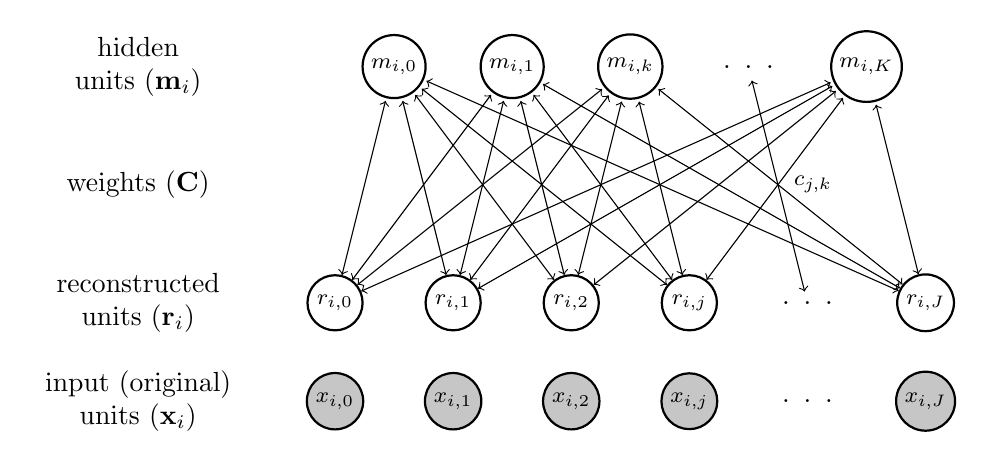
\begin{tikzpicture}[shorten <=1pt,<->,draw=black!100]
	\def \rowtwoht{4.25cm}
	\def \weightlevel{2.75cm}
	\def \rowoneht{1.25cm}
	\def \basement{0cm}
	\tikzstyle{m-node}=[circle,draw=black!100,thick,inner sep=2pt,minimum size=7mm]
	\tikzstyle{r-node}=[circle,draw=black!100,thick,inner sep=2pt,minimum size=7mm]
	\tikzstyle{d-node}=[circle,draw=black!100,fill=gray!45,thick,inner sep=2pt,minimum size=7mm]
	\tikzstyle{dots}=[text width=5ex, text centered]
	\tikzstyle{annot}=[text width=17ex, text centered]
	% labels
	\node[annot] (hidden-layer) at (0cm,\rowtwoht) {hidden units ($\mathbf{m}_i$)};
	\node[annot] (weights) at (0cm,\weightlevel) {weights ($\mathbf{C}$)};
	\node[annot] (r-layer) at (0cm,\rowoneht) {reconstructed units ($\mathbf{r}_i$)};
	\node[annot] (d-layer) at (0cm,\basement) {input (original) units ($\mathbf{x}_i$)};
	
	\node[dots] 	(m3)	at (7.75cm,\rowtwoht)	 	{. . .};
	\node[dots] 	(r4) 	at (8.5cm,\rowoneht)   		{. . .};
	\node[dots] 	(d4) 	at (8.5cm,\basement)   		{. . .};
	
	\footnotesize
	% hidden layer
	\node[m-node] 	(m0)	at (3.25cm,\rowtwoht)		{$m_{i,0}$};
	\node[m-node] 	(m1)	at (4.75cm,\rowtwoht)		{$m_{i,1}$};
	\node[m-node] 	(m2)	at (6.25cm,\rowtwoht)	 	{$m_{i,k}$};
	\node[m-node] 	(m4)	at (9.25cm,\rowtwoht)	 	{$m_{i,K}$};
	
	% reconstructed vector
	\node[r-node] 	(r0)	at (2.5cm,\rowoneht)		{$r_{i,0}$};
	\node[r-node] 	(r1)	at (4cm,\rowoneht)		{$r_{i,1}$};
	\node[r-node] 	(r2)	at (5.5cm,\rowoneht)	 	{$r_{i,2}$};
	\node[r-node] 	(r3)	at (7cm,\rowoneht) 		{$r_{i,j}$};
	\node[r-node] 	(r5) 	at (10cm,\rowoneht)   		{$r_{i,J}$};
	%\node[r-node] 	(r6) 	at (9.75cm,\rowoneht)   	{$r_{i,J}$};
	
	% data vector
	\node[d-node] 	(d0)	at (2.5cm,\basement)		{$x_{i,0}$};
	\node[d-node] 	(d1)	at (4cm,\basement)		{$x_{i,1}$};
	\node[d-node] 	(d2)	at (5.5cm,\basement)	 	{$x_{i,2}$};
	\node[d-node] 	(d3)	at (7cm,\basement) 		{$x_{i,j}$};
	\node[d-node] 	(d5) 	at (10cm,\basement)   		{$x_{i,J}$};
	%\node[d-node] 	(d6) 	at (9.75cm,\basement)   	{$x_{i,J}$};
	
	\path 
		(m0)	edge	node	{}	(r0)
		(m0)	edge	node	{}	(r1)
		(m0)	edge	node	{}	(r2)
		(m0)	edge	node	{}	(r3)
		(m0)	edge	node	{}	(r5)
		
		(m1)	edge	node	{}	(r0)
		(m1)	edge	node	{}	(r1)
		(m1)	edge	node	{}	(r2)
		(m1)	edge	node	{}	(r3)
		(m1)	edge	node	{}	(r5)
		
		(m2)	edge	node	{}	(r0)
		(m2)	edge	node	{}	(r1)
		(m2)	edge	node	{}	(r2)
		(m2)	edge	node	{}	(r3)
		(m2)	edge	node	{}	(r5)
		(m3)	edge	node[right=1mm]	{$c_{j,k}$}	(r4)
		%	
		(m4)	edge	node	{}	(r0)
		(m4)	edge	node	{}	(r1)
		(m4)	edge	node	{}	(r2)
		(m4)	edge	node	{}	(r3)
		(m4)	edge	node	{}	(r5);
		
\end{tikzpicture}
%\end{center}
\caption{Restricted Boltzmann Machine} 
\label{fig:rbm}
%\end{mdframed}
\vspace{12pt}
\end{mdframed}
\end{figure}

\paragraph{Form.}
MCMMs and RBMs are both bipartite graphs, whereas the classical autoencoder is 
not (see the description of bipartite graphs in chapter~\ref{ch:graph}).
The classical autoencoder, shown in figure~\ref{fig:autoencoder}, has distinct input 
and output layers.
Each original data vector $\textbf{x}_i$ enters the network at the input layer, is compressed 
at $\textbf{m}_i$, and reconstructed at $\textbf{r}_i$. Because there are three layers 
of nodes in an autoencoder, there must be two layers of weights ($\textbf{A}$ and $\textbf{B}$ in figure~\ref{fig:autoencoder}), both which are oriented in the same direction \citep{baldi:2012}.
Classical autoencoders thus function similarly to supervised feed-forward neural networks. 
In fact, the only difference between a classical autoencoder and a supervised 
feed-forward network is that a classical autoencoder's target vectors are its input vectors \citep{bourlard:1988}. 

By contrast, both MCMMs and RBMs lack an input layer that is distinct from the reconstruction layer. 
In both MCMMs and RBMs,
the original (input) data vectors $\textbf{x}_i$ are actually not even part of the graph, 
since there are no weights (i.e., arcs) that connect the original data vectors to the other 
vectors (namely, the hidden and reconstruction node layers). %\citep{martens:2013}
Speaking strictly in terms of form, therefore, MCMMs and RBMs belong together in a 
class that excludes the classical autoencoder.

\paragraph{Node Activation.} The RBM and classical autoencoder essentially use the same function for computing node activities, namely the \emph{sigmoidal weighted sum} \citep{hinton:1987trans, hinton-and-salak:2006}.
%are essentially the same, generally  sharing the same activation function.
However, MCMMs, as we shall see, call for a different type of activation function, a type of function that \citet{saund:94} calls a \emph{mixing function}.
% that has different properties to those of sigmoidal weighted sum.
The sigmoidal weighted sum is a composition of two functions: the ``outer'' function is the logistic sigmoid, 
	\begin{equation} %\label{eq:sigws}
	\label{eq:sig}
	\sigma(t) = \frac{1}{1 + e^{-t}} 
	\end{equation} %\label{eq:sigws
The ``inner'' function replaces the $t$ in equation~\eqref{eq:sig}. It is a weighted-sum of the form 
\begin{equation} \label{eq:wtd-sum}
t = \sum_{j} x_{j} w_{j,k} \qquad  \text{or, equivalently,} \qquad t = \textbf{x}^{\textsf{T}}\textbf{w}_k
\end{equation}
%$\sum_{j} x_{j} w_{j,k}$, which is equivalent to the \emph{inner product} of vectors $\textbf{x}$ and  $\textbf{w}$, that is, $\textbf{x}^\textsf{T}\textbf{w}_k$, 
where $\textbf{x}$ is a vector of $J$ node activities, and $\textbf{w}_k$ is a vector of $J$ weights. These weights connect the nodes of $\textbf{x}$ to a particular node (namely, the $k$th node) in a \emph{different} layer, which we will call $\textbf{m}$. 
The logistic sigmoid \eqref{eq:sig} maps the weighted sum (no matter how large or small it may be) to a number in the interval $[0,1]$, thus constraining node activities to this interval.
%	\begin{equation} %\label{eq:sigws}
%	\label{eq:sig}
%	\sigma(x) = \frac{1}{1 + e^{-x}} 
%	\end{equation} %\label{eq:sigws
Thus, in a classical autoencoder the activity of each the hidden node $m_k$ is computed by equation~\eqref{eq:sig-m-ac}. 
%That is, a weighted sum of the input layer's activities is fed to the sigmoid function \citep{bourlard:1988}.
\begin{align}
\label{eq:sig-m-ac}
m_{k} &= \sigma\big(\sum_{j} x_{j} a_{j,k}\big) \\
%m_{i,k} = P(m_{i,j}|r_{i,j}) =\sigma\big(\sum_{j} c_{j,k} r_{i,j}\big)
\label{eq:sig-r-ac}
%r_{i,j} = P(r_{i,j}|m_{i,k})  = \sigma\big(\sum_{i,k} c_{j,k} m_{i,k}\big)
r_{j} &= \sigma\big(\sum_{k}  m_{k} b_{k,j} \big)
\end{align}
For example, to obtain the activity of the hidden node $m_{i,2}$.
we compute $\sum_{j} x_{i,j} a_{j,2}$, where each $x_{i,j}$ is the activity of one of the $J$ nodes in the $i$th input vector $\textbf{x}_i$, and $a_{j,2}$ is the the weight connecting the $j$th node in $\textbf{x}_i$ to the hidden node $m_{i,2}$ (see figure~\ref{fig:autoencoder}).
%, which is the equivalent to the inner product \textbf{x}_i \cdot \textbf{c}^{\textsf{T}}_4$ 
We then feed the resulting sum to the sigmoid function, thereby obtaining an activity for $m_{i,2}$ that is within $[0,1]$. 
We do the same for each hidden node in $\textbf{m}_i$
The process is the same for the reconstruction nodes, except that the just-computed hidden-node activities now become the input values, and the matrix $\textbf{B}$ now supplies the weight vectors instead of $\textbf{A}$.

An RBM is can almost be described as an autoencoder in bipartite form. There are a few differences, however, as we will soon see.
%\citep{hinton-and-salak:2006}. 
The activation functions of an RBM are presented below as equations \eqref{eq:sig-m} to \eqref{eq:sig-m-sample}, where $\delta$ and $\theta$ are biases,\footnote{Another ostensible difference 
is the presence of the biases in the 
RBM activation functions. However, some authors, e.g., \citet{rudy-and-taylor:2014}, have included biases in the activation functions of classical autoencoders.} and $\hat{m}_k$ and $\hat{r}_j$ denote preliminary activation values for the $k$th hidden unit and the $j$th surface unit, respectively.
\begin{align}
\label{eq:sig-m}
%m_{k} &= \sigma\big(\sum_{j} r_{j} c_{j,k} + \delta_{j}\big) \\
%\label{eq:sig-m-sample}
%m_{k} &= \sigma\big(\sum_{j} r_{j} c_{j,k} + \delta_{j}\big) \\
%p(h_{k}=1|\mathbf{v}) &= \sigma\big(\sum_{j} r_{j} c_{j,k} + \delta_{j}\big) \\
\hat{m}_k \,\, &= \,\, p(m_{k}=1 \, | \, \mathbf{r}) \,\, = \,\, \sigma\big(\sum_{j} r_{j} c_{j,k} + \delta_{j}\big) \\
\label{eq:sig-m-sample}
%p_{k} &= \sigma\big(\sum_{j} r_{j} c_{j,k} + \delta_{j}\big) \\
%m_{k} &= \text{rand}_{\textsc{BERN}}\Big(p(m_{k}=1\,\,|\,\,\mathbf{r})\Big)
m_{k}\,\, &= \,\, \text{rand}_{\textsc{BERN}}(\hat{m}_k)
\end{align}
\begin{align}
\label{eq:sig-r}
\hat{r}_k \,\, &= \quad p(r_{j}=1 \, | \, \mathbf{m}) \,\, =  \,\, \sigma\big(\sum_{k}  m_{k} c_{k,j} + \theta_{k}\big) \\
\label{eq:sig-r-sample}
%r_{j} &= \text{rand}_{\textsc{BERN}}\Big(p(r_{j}=1\,\,|\,\,\mathbf{m})\Big)
r_{j} \,\, &= \,\, \text{rand}_{\textsc{BERN}}(\hat{r}_k)
\end{align}
Equations~\eqref{eq:sig-m} and \eqref{eq:sig-r} are basically the same as the classical autoencoder's activation functions. 
However, one of the differences between RBMs and  classical autoencoders is that RBMs require the real-number outputs of the logistic sigmoid function to be mapped to either the 0 or 1 \citep{hinton:2012}.
%; that is, it requires strictly binary hidden and surface units. This is accomplished 
RBMs accomplish this strict boolean mapping by treating each sigmoidal output as  the \emph{probability of getting a successful outcome} from a Bernoulli trial, where a ``successful outcome'' is a valuation of 1, as in $m_k = 1$ and $r_j = 1$). Thus, equation~\eqref{eq:sig-m} computes the probability $\hat{m} = p(m_{k}=1|\mathbf{r})$, the probability that the $k$th hidden unit is 1 given the surface-unit activities $\mathbf{r}$. Similarly, \eqref{eq:sig-m} computes $\hat{r}_k = p(r_{j}=1|\mathbf{m})$, the probability that $j$th surface unit is 1 given the hidden-unit activities. We use $\hat{\mathbf{m}}$ and $\hat{\mathbf{r}}$, respectively, to denote the vectors that comprise the individual probabilities
$\hat{m}_k \text{for} k \in K$ and $\hat{r}_j \text{for} j \in J$.
%equations~\eqref{eq:sig-m-sample} and \eqref{eq:sig-r-sample} 
%via 
%applying 
The probabilities in these vectors are then passed to the Bernoulli random sampling function $\text{rand}_{\textsc{BERN}}$, which outputs 1 or 0 for each component. In particular, 
$\text{rand}_{\textsc{BERN}}(h_k)$ outputs 1 at a probability of $h_k$ (i.e., $h$\% of the time), and if it 
does not output 1, it outputs 0. Likewise, $\text{rand}_{\textsc{BERN}}(v_j)$ outputs 1 at probability $v_j$.
%$\text{rand}_{\textsc{BERN}}(v_j)$. which, for each individual probability $h_k$ or $v_j$, randomly chooses 1 at probability   out of the set $\{\,0,\,1\}$
%which randomly chooses $1$ according to it
%the binomial sampling function $\text{rand}_{\textsc{BERN}}$, which samples outcomes from a binomial distribution.

%these equations \eqref{eq:sig-m} and \eqref{eq:sig-r} do not calculate actual activities, but preliminary activities, i.e., the components of vectors  $\mathbf{h}$ and $\mathbf{v}$. These preliminary values are in fact \emph{probabilities}. That is, $h_k$ is the probability $p(h_{k}=1|\mathbf{v})$, i.e., the probability that the $k$th unit of the hidden vector $\mathbf{h}$ is 1 given the present activities of the surface (or visible) vector $\mathbf{r}$,  and 
%and $\eqref{eq:sig-r} calculates$v_j$ is the probability $p(r_{j}=1|\mathbf{h})$, that is, the probability that the $j$th unit in the surface vector is 1 given the present activities in hidden vector $\mathbf{m}$.
%\begin{table}[!h]
%\begin{tabular}{ll}
%\centering
%\makecell{$p(r_{j}=1|\mathbf{h})$} & \makecell{the probability that the $j$th unit in the surface vector is 1 \\ given the present activities in hidden vector $\mathbf{m}$} \\
%\end{tabular}
%\end{table}
%An additional step is necessary to realize the actual activities from the values in $\mathbf{h}$ and $\mathbf{v}$.
%One of the ways in which an RBM differs from a classical autoencoder is that it requires the real-number outputs of the logistic sigmoid function to be mapped to either 0 or 1. This is accomplished in equations~\eqref{eq:sig-m-sample} and \eqref{eq:sig-r-sample} via the binomial sampling function $\text{rand}_{\textsc{BINOM}}$, which takes two parameters, namely the input $n$, the number of the trials, and the (conditional) probability that a given trial should yield a ``successful outcome'' (i.e., a value of 1 for the variable in question). 

Consider, for example, the preliminary hidden-unit vector 
\begin{equation}
\mathbf{h} \quad = \quad [ \,  0.1,  \,  0.9,  \,  1 ,  \,  0.5, \,  0.5,  \,  0.5  \, ]
\end{equation}
That is, the probability that $h_0 = 1$ is 0.1, and so on. 
%the probability that $h_1 = 1$ is 0.9, and so on. %
These values came from the logistic sigmoid, as shown in equation \eqref{eq:sig-m}.
We apply the function $\text{rand}_{\textsc{BERN}}$ to vector $\mathbf{h}$ to obtain the final hidden-unit activations:
\begin{equation}
\mathbf{m} \,\,\, =  \,\,\,   \text{rand}_{\textsc{BERN}}(\mathbf{h})  \,\,  =  \,\,   [ \, 0, \, 1, \, 1, \, 1, \, 0, \, 0 \,]
\end{equation}
Note, however, that each component in $\mathbf{m}$ is \emph{randomly} sampled given the probabilities in 
$\mathbf{h}$. These values are thus not deterministic.
%But note that is just one possible outcome for the vector $\mathbf{m}$; i.e., it is the output of a single as the number of trials $n$ is just 1. Another trial might produce 
If we should run $\text{rand}_{\textsc{BERN}}$ again, we might get $[0, 0, 1, 1, 0, 0]$ or $[0, 1, 1, 0, 0, 0]$, etc.  %Each component is randomly sampled given the probabilities in $\mathbf{h}$.

%~\eqref{eq:sig-m-sample}  The final activity $m_{k}$ of a hidden unit must be either 1 or 0.  The in an RBM, the final hidden and surface-unit activities $\mathbf{m}$ and $\mathbf{r}

%These are clearly similar to the classical autoencoder's activation 
%functions~\eqref{eq:sig-m-ac} and \eqref{eq:sig-r-ac},
%but there are a few differences.  %but the classical encoder could in principle accomodate biases \citep{song:2013}   But the 
Another important difference between
RBMs and classical autoencoders is that the RBM's functions~\eqref{eq:sig-m} and \eqref{eq:sig-r} 
both refer to the same weight matrix $\textbf{C}$, whereas the classical 
autoencoder's  functions \eqref{eq:sig-m-ac} and \eqref{eq:sig-r-ac} each 
refer to a different weight matrix 
($\textbf{A}$ in equation~\eqref{eq:sig-m-ac} and $\textbf{B}$ in equation~\eqref{eq:sig-r-ac}). 
An RBM's learning process is thus bi-directional: 
The hidden-unit activities are conveyed to the reconstruction 
units via the weight matrix $\textbf{C}$, and then the reconstruction 
activities are conveyed back to the hidden units via the same weight matrix, resulting in a cyclic process.
 
%\citep{larochelle-and-bengio:2008}. 

But despite these differences, RBMs and classical autoencoders can be grouped together where activation functions are concerned, since they both use the sigmoidal weighted sum.
The sigmoidal weighted sum is a very common activation function in neural networks, 
but it is not the only way to compute the activity of a node. Any activation function, to borrow
an analogy from \citet{saund:94}, is essentially a voting rule, that is,  a policy 
for combining multiple input votes into a single output decision.  
In the context of neural-network models such as RBMs, MCMMs, and 
classical autoencoders, the output decision takes the form of a \emph{node activity},
and the input votes are the \emph{weighted} activities of the preceding layer's nodes. 
That is, each vote is a product of the form $x_{j} w_{j,k}$, where $x_{j}$ is the activity 
of the $j$th node in a given layer of nodes, and $w_{j,k}$ is the weight associated with that 
node. The question being voted upon is the activity of the $k$th node in the 
\emph{next} layer, and there are
a total of $J$ votes to consider.

The sigmoidal weighted sum is in effect a sort of average and thus tends to obscure
the influence of minority subsets of inputs. \citet{saund:94} argues 
that the averaging nature of the sigmoidal weighted sum is inappropriate when one wants to encourage
a small subset of votes to take responsibility for a given surface unit's activity, as in MCMMs.
He thus proposes for MCMMs a special kind of activation function called a \emph{mixing function}.
We discuss the properties of mixing functions in 
section~\ref{sec:mixing-function}.

\paragraph{Optimization procedure.}  In a classical autoencoder, the two layers of 
weights---first $\textbf{B}$ and then $\textbf{A}$---are directly updated via 
back-propagation \citep{rumelhart-et-al:1985, hinton:1987, hinton:1987trans, bourlard:1988}.
The values of the hidden units are not directly manipulated; rather, they change  
only as a 
consequence of the adjustments made to the weights. The same is true in an RBM: 
an RBM's hidden-unit activities change in response to adjustments 
made to the weights and biases, but they are not
adjusted directly.

In an MCMM, by contrast, both $\textbf{m}_i$ and $\textbf{C}$ are directly manipulated. This means that
an MCMM's learning process begins with two unknown variables, the matrices $\textbf{M}$ and 
$\textbf{C}$, and it must induce both during the course of learning. We will discuss how an MCMM accomplishes this---that is, how it learns---in section~\ref{sec:two-in-one}.
%That is, an MCMM requires two complimentary process, \textsc{Optimize-M} 
%and \textsc{Optimize-C} (see section~\ref{sec:num-opt}), each directly manipulating 
%the values in its respective matrix. 

\subsection{Mixture and Mixed-Membership Models}
\label{sec:mixture-models}
A mixture model attempts to account for the data points in a data set 
by assuming that multiple probability
distributions are responsible for generating the data. 
It also assumes that \emph{exactly one}
of these underlying distributions is responsible for each data point \citep{bishop:2006}. 
 These underlying 
distributions can be interpreted as clusters. Under this interpretation, each data point is 
is assigned to a cluster (distribution) that is responsible for 
generating it \citep{fraley:1998}. 
However, since the process is probabilistic,
data points are often not mapped to clusters with 100 percent certainty. 
There may be, for example, a 60 percent chance that a given data point belongs to one 
cluster, a 30 percent chance it belongs to another, and a 10 percent chance 
it belongs to yet another. In a \emph{hard clustering}, the data point is 
assigned to the single most probable category, and the other less probable 
possibilities are forgotten. However, the uncertainty can also be left 
unresolved, so that, in the case of our example, all three possibilities, 
along with their respective likelihoods, would be returned. This is a 
\emph{soft clustering}. But even in the case of a soft clustering, 
we still assume that the data point in question \emph{fundamentally} 
belongs to only one cluster; 
the ``softness'' of the clustering just expresses the model's uncertainty 
as to which cluster this is. %the data point belongs.

By contrast, a mixed-membership model, e.g., Latent Dirichlet Allocation \citep{blei-et-al:2003},
%\footnote{
%Like latent Dirichlet allocation, MCMMs have
%been applied to document classification; \cite{sahami-et-al:96} 
%use an MCMM to group $I$ documents into $K$ clusters.  Documents are 
%represented as vectors $\mathbf{x}_i$ of $J$ features. The features, i.e. surface units, 
%each indicate the absence or presence of a particular word (cf. the $\mathbf{x}$ 
%vector in figure~\ref{fig:mcmm}). The topics in \cite{sahami-et-al:96} are represented 
%as the MCMM's hidden units $\mathbf{m}_i$. Documents are grouped into topic 
%clusters by the learning process described below in section~\ref{sec:mcmm-learning}.}, 
views each data point as a complex object, that is, as an object that itself consists of multiple objects, 
\emph{each of which} is generated by one of multiple probability distributions (or clusters) \citep{airoldi-et-al:2014}. 
For example, in a mixed-membership topic model, the complex objects are the 
\emph{documents} within a given corpus. The elemental objects that compose 
the documents are \emph{words}. The clusters correspond to \emph{topics}, which generate 
the words that together compose the documents. That is, each document is a set of words, and each 
word is generated by a particular topic. The document is associated to 
(or ``becomes a member of'') each topic that is
responsible for at least some of its words. 

However, these topics (if more than one topic is involved) cannot all claim equal responsibility
for the document in question. One topic might be responsible for 40 percent of the words, for instance, 
and another for 30 percent, and so on. 
%A single topic 
%cannot be responsible for the whole document unless no other topics 
%are involved.  
It is important to note that these percentages 
do not indicate uncertainty as they would in mixture models. 
%The assumption
%of multiple causes (i.e., clusters) is built 
%into mixed-membership models, whereas mixture models assume a single cause for each 
%data object. 
The reason that mixed-membership models yield percentages is 
that they decompose each data object into many elemental objects and allow different 
causes (e.g., topics) to claim responsibility for different 
elemental objects within the same document. 

Like mixed-membership models, multiple-cause mixture models (MCMMs) 
allow multiple causes to take part in accounting for a single data point. 
That is, as in mixed-membership models, MCMMs provide a means for 
different causes to take responsibility for different parts of a data point. 
Thus, both MCMMs and mixed-membership models transcend the single-cause assumption of standard 
mixture models.
% and their assumption that each data point ultimately has 
%only one cause.

At the same time, however, MCMMs differ from mixed-membership models in that MCMMs do not deal in 
percentages of any sort.
%; that is, in MCMMs, a cause (or cluster) cannot be, for instance, 
%40 percent responsible for a (complex) data object. Rather, in MCMMs,
In MCMMs, 
cluster membership is always binary: either True or False. %, 0 or 1---100 percent or 0 percent, as it were. 
This behavior is a consequence of the nature of \emph{mixing functions}, the activation functions of MCMMs (see section~\ref{sec:mixing-function}). 
While MCMMs do allow individual clusters to claim responsibility 
for particular features, they ultimately do not attribute different proportions of a given feature vector
to different clusters. In an MCMM, as long as at least one feature is caused by a given cluster, the \emph{whole} feature
vector (or data point) is assigned to that cluster. It is also wholly assigned to any a cluster that is responsible for one or more of its features. 
%(i.e., individual components within data points). This is in fact a key property of MCMMs. 
%The difference between MCMMs and mixed-membership models stems from 
%both the neural nature and the mixing functions MCMMs: An MCMM's mixing 
%function requires a hidden unit's activity to be 1 in order for it count as an 
%``\textsc{on}'' vote for a particular surface unit, and 0 to be an ``\textsc{off}'' vote. 
%Of course, during learning, many hidden-unit activities will be between 0 and 1, 
During learning, many hidden-unit activities will be between 0 and 1,
but the learning process pushes them ever closer to one of these two values. 
Activity values between 0 and 1 can be interpreted as ``almost off'' or ``almost on,'' depending on where exactly they lie in this interval,
but not as real percentages as in mixed-membership models. 

This binary treatment 
%of causes 
is arguably more suitable for
morphological learning than a framework in which ``ownership percentages'' are assigned to causes.
We generally do not think of words' morphological compositions in 
terms of percentages.  That is, we tend not to say things like, ``60 percent 
of this word belongs to this morphological category, and 40 percent belongs 
to that category.'' Of course, such a statement would be particularly incoherent 
if we were speaking in terms of morphosyntactic categories, such as past tense. 
But it is also problematic in the case of form-based categories. Proportions or percentages of elemental components
do not have coherent interpretations in morphology as they do in topic modeling.
%of characters (or form-describing binary features) simply do not  
%meaning in morphology, not as one comparable to the that of word proportions 
%in topic modeling, at any rate. 
In morphology, it is the simple presence/absence 
of a morphological unit that is important, not the proportion of characters 
or features it can claim. Moreover, the percentages of mixed-membership 
models correspond to degrees of membership:
\begin{quote}\noindent 
[M]ixed membership models assume that individuals or observational units 
[i.e., words] may only partly belong to population mixture categories [i.e., topics] \dots. 
The degree of membership then is a vector of continuous, 
non-negative latent variables [i.e., hidden units] that add up to 1 \citep[][p. 4]{airoldi-et-al:2014}. 
\end{quote}
By contrast, in morphology, there are no degrees of membership (and thus
no a requirement that they should add up to one).

%\begin{table}[htb]
%\centering
%\begin{tabular}{ccc}
%Topic-Modeling & & ULM \\
%document & $\to$ & word \\
%topic & $\to$ & morph/morpheme \\
%word & $\to$ & word-internal feature or character \\
%\end{tabular}
%\caption{Some topic-modeling terms and their ULM equivalents. That is, for instance, \emph{documents}
%in the context of topic modeling are equivalent to \emph{words} in the context of the unsupervised learning
%of morphology.}
%\label{tab:tm-to-ulm}
%\end{table}	
				
\section{Mixing Function}
\label{sec:mixing-function}

In this section, we discuss the \emph{mixing function}, 
the component within an MCMM responsible for determining 
activities of the surface nodes in $\textbf{r}_i$.
A mixing function takes as input the hidden-unit activities $\textbf{m}_i$ accompanied by a vector of weights  
linking the hidden units to a particular surface node. It then outputs the activity 
of this surface node. 
%and their corresponding weights is  multiplied by 
%particular vector weights---and outputs the activity of a particular surface 
%(or reconstruction) node. 
\citet{saund:94} describes mixing functions as
\emph{voting rules}, i.e., rules whereby multiple votes are combined in some way to yield a single decision, 
Each vote is a product of the form $m_{i,k}c_{j,k}$ for $k \in K$, and the decision is a single node activity. 

Mixing functions are 
activation functions that are specially tailored to serve the needs of MCMMs. 
These needs are as follows:
\begin{enumerate}
\item Hidden-unit activities 
must be interpretable as binary indicators of cluster membership, where $1$ 
indicates membership, and $0$ non-membership. Thus, in the case of 
Multimorph, a given word belongs to the 
$k$th cluster if its $k$th hidden-unit activity is $1$.
\item Each column in the matrix $\textbf{C}$ must be interpretable as the centroid 
(or ``average'' vector) of a particular cluster. That is, the $k$th column 
$\textbf{C}$ (whose dimensions are $J \times K$) must be interpretable as the centroid vector of the $k$th cluster. This means that the $j$th element in the $k$th column of $\textbf{C}$ must be interpretable as the average $j$th feature value across the data points that belong to the $k$th cluster. 

\end{enumerate}
In short, both the hidden-unit values and weights must have coherent interpretations. 
%As mentioned in , section~\ref{sec:context}
The sigmoidal weighted sum
does not satisfy this criterion, since it does not encourage its 
parameters to take on interpretable valuations (see section~\ref{sec:context}). It is therefore 
not a mixing function, even though it is an activation function.  All mixing functions
are activation functions, but not all activation functions are mixing functions.

Just as there are many possible activation functions, there are many 
possible mixing functions.
\citet{saund:94} proposes two, each designed 
to suit a particular data domain.  The two data domains, namely 
the ``\textsc{write-black}'' and ``\textsc{write-white-and-black}'' 
domains, are distinguished by the nature of the voting task that 
determines the activities of surface nodes. 
In the \textsc{write-black} domain, the decision in question is 
 whether a given surface unit should be ``black'' (i.e., 1) or ``not black'' (i.e., 0). 
 The individual votes, as in the case of the sigmoidal activation function (see section~\ref{sec:context}), are products of the form $m_{i,k} c_{j,k}$,
 where $m_{i,k}$ is the $k$th hidden unit's activity and $c_{j,k}$ is its weight.
The mixing function in the \textsc{write-black} domain, the function that combines these votes,
 %for each such decision are 1 or 0 (or between 1 and 0 prior to convergence) 
 %and combined according to the  
 is the Noisy-OR function \citep{pearl:1988}, defined as follows:
% defined in \eqref{eq:noisy-or}.
\begin{equation}\label{eq:noisy-or}
r_{i,j} = 1 - \prod\limits_{k} (1 - m_{i,k} c_{j,k})
\end{equation}
 The Noisy-OR function is essentially an \textit{OR} gate, or, to put it another way, 
 an ``at-least-one'' gate. That is, the surface node $r_{i,j}$ is $1$ (and thus ``\textsc{on}'') as long as 
 \emph{at least one} vote (or cause) is active.
%Increasing the number of active votes beyond 1 does not further increase the activity of $r_{i,j}$: If more than one vote is active,
%$r_{i,j}$ is still going to be $1$. The activity , the number of active votes does not matter, as long as 
Thus, the output of Noisy-OR does not increase
as the number of active causes increases beyond 1; it is 1 as long as there is at least one active cause (or ``yes'' vote).

The \textsc{write-white-and-black} domain differs from \textsc{write-black} 
in that it requires the mixing function to be capable of outputting negative surface-unit 
activities as well as positive, that is, values ranging from $-1$ to $1$.
Clearly, the Noisy-OR function does not satisfy this requirement.
Saund thus proposes the following mixing function for the \textsc{write-white-and-black} domain.
 \begin{align}\label{eq:wwb}
  r_{i,j} &=
    \begin{cases}
    %\label{eq:wwb-top}
      \frac{\sum\limits_{k} m_{i,k} c_{j,k}}{\sum\limits_{k} m_{i,k} |c_{j,k}|} & \text{$\forall m_{i,k}, c_{j,k} : m_{i,k} c_{j,k} \in \{-1,0,1\}$} \\
      %\label{eq:wwb-bottom}
      0 & \text{if \, $\sum\limits_{k} m_{i,k} |c_{j,k}|= 0$} 
    \end{cases}
 \end{align}
where 
\begin{center}
$-1 \leq c_{j,k} \leq 1$  \\
$0 \leq  m_{i,k} \leq  1$\\
$-1 \leq  r_{i,j} \leq  1$ 
\end{center}
and the components $x_{i,j}$ of the original data points
are each either $1$ or  $-1$. Note the absolute value in the denominator in the 
upper case of equation~\eqref{eq:wwb}. 
This absolute value allows the numerator and denominator to differ in sign so that 
the $r_{i,j}$ can be either positive or negative (and thus match the signs of the components of the original data points).

 Notice also that equation~\eqref{eq:wwb} contains weighted sums. In fact, the weighted sum
in the numerator of the upper case of equation~\eqref{eq:wwb} is the same weighted sum that appears in the sigmoidal weighted sum, namely $\sum\limits_{k} m_{i,k} c_{j,k}$.
 Nevertheless, there are important differences 
 between equation~\eqref{eq:wwb} and the sigmoidal weighted sum. First, there is 
 no logistic sigmoid in equation~\eqref{eq:wwb}; it is the denominator $\sum_{k} m_{i,k} |c_{j,k}|$ 
 that constrains output of \eqref{eq:wwb} to the interval $[-1,1]$. The other 
 difference is that the nonlinearity arises from the conditions on the output \eqref{eq:wwb}; 
 to avoid division by zero, it is necessary to stipulate that $r_{i,j}=0$ if 
 $\sum_{k} m_{i,k} |c_{j,k}| = 0$, a result that occurs only if every vote is 0, 
 in which case no cluster can claim responsibility for the value of $r_{i,j}$. But 
 because $0$ never occurs in the original data points in the \textsc{write-white-and-black} 
 domain, the learning process would tend to drive activities of the reconstruction nodes 
 away from $0$. That is, because the learning process seeks to minimize the discrepancy 
 between $\textbf{r}_i$ and $\textbf{x}_i$, $0$ cannot be a valid final value for any $r_{i,j}$.  
 Thus, the weights and the hidden-unit vectors will be shaped to produce surface-node 
 activities that are either $-1$ or $1$ in accordance with the component values of 
 the original data points. 

To ensure that the activity of $r_{i,j}$ is either $-1$ or $1$, at least one hidden 
unit $m_{i,k}$ must have an activity of 1, and the weight associated with this 
hidden unit, namely $c_{j,k}$, must be either $-1$ or $1$. This would associate 
the surface unit $r_{i,j}$ to at least one cluster. Ultimately, mixing 
function \eqref{eq:wwb} encourages hidden-unit activities to move toward 
either $0$ or $1$ and the weights toward either $-1$ and $1$. These are 
values with clear cluster-oriented interpretations: The $1$s and $0$s of the 
hidden-unit vector indicate cluster membership and nonmembership, respectively, 
while the weights adopt the same values, namely $\{-1, 1\}$ present in the original data points. 
This is important, since, as noted above, an MCMM's weight vectors have to be 
interpretable as composite or average vectors for the clusters.

In preliminary experiments for the present work, I tried both the Noisy-OR 
and the \textsc{write-white-and-black} mixing function. The latter did 
not work well; in fact, under the \textsc{write-white-and-black} mixing function, the system 
failed to make progress toward learning to reconstruct the original 
data points. This may have been due to the sparseness of the data points 
in this study; each data point is a vector of hundreds of feature slots, but 
only a handful have the value $1$.
%There are hundreds of features, and each has a designated slot in each feature vector.
(We will discuss these features in detail in chapter~\ref{ch:experi}.)

In a \textsc{write-black} formulation, absent features have the value $0$, but in the\textsc{write-white-and-black} formulation, they are $-1$. Therefore, in a sparse feature vector under the\textsc{write-white-and-black} formulation, the vast majority of features are $-1$. The cumulative effect of all these negatives in \eqref{eq:wwb} seemed to drown out the few positive features, making it impossible to reproduce the original data vectors. 

Noisy-OR, on the other hand, did allow learning to take place; that is, 
the system was able to reduce its error with Noisy-OR as its mixing function. 
Apparently, this study's sparse feature vectors (i.e., data points) are more aptly 
placed in the \textsc{write-black} domain than the \textsc{write-white-and-black} domain.

\begin{figure}[t]
\begin{mdframed}
%\begin{center}
\centering
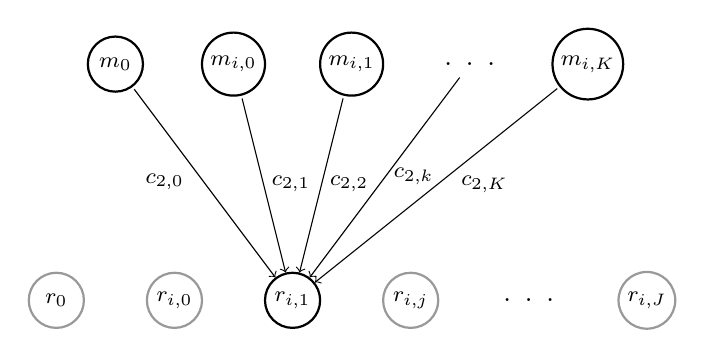
\begin{tikzpicture}[shorten <=1pt,->,draw=black!100]
	\def \rowtwoht{4.25cm}
	\def \weightlevel{2.75cm}
	\def \rowoneht{1.25cm}
	\def \basement{0cm}
	\tikzstyle{m-node}=[circle,draw=black!100,thick,inner sep=2pt,minimum size=7mm]
	\tikzstyle{r-node}=[circle,draw=black!100,thick,inner sep=2pt,minimum size=7mm]
	\tikzstyle{r-node-2}=[circle,draw=black!40,thick,inner sep=2pt,minimum size=7mm]
	%\tikzstyle{d-node}=[circle,draw=black!100,fill=gray!45,thick,inner sep=2pt,minimum size=7mm]
	\tikzstyle{dots}=[text width=5ex, text centered]
	%\tikzstyle{annot}=[text width=17ex, text centered]
%	% labels
%	\node[annot] (hidden-layer) at (0cm,\rowtwoht) {hidden units ($\mathbf{m}_i$)};
	%\node[annot] (weights) at (0cm,\weightlevel) {weights ($\mathbf{C}$)};
%	\node[annot] (r-layer) at (0cm,\rowoneht) {reconstructed units ($\mathbf{r}_i$)};
	%\node[annot] (d-layer) at (0cm,\basement) {input (original) units ($\mathbf{x}_i$)};
	
	\node[dots] 	(m3)	at (7.75cm,\rowtwoht)	 	{. . .};
	\node[dots] 	(r4) 	at (8.5cm,\rowoneht)   		{. . .};
	%\node[dots] 	(d4) 	at (8.5cm,\basement)   		{. . .};
	
	\footnotesize
	% hidden layer
	\node[m-node] 	(m0)	at (3.25cm,\rowtwoht)		{$m_0$};
	\node[m-node] 	(m1)	at (4.75cm,\rowtwoht)		{$m_{i,0}$};
	\node[m-node] 	(m2)	at (6.25cm,\rowtwoht)	 	{$m_{i,1}$};
	\node[m-node] 	(m4)	at (9.25cm,\rowtwoht)	 	{$m_{i,K}$};
	
	% reconstructed vector
	\node[r-node-2] 	(r0)	at (2.5cm,\rowoneht)		{$r_0$};
	\node[r-node-2] 	(r1)	at (4cm,\rowoneht)		{$r_{i,0}$};
	\node[r-node] 	(r2)	at (5.5cm,\rowoneht)	 	{$r_{i,1}$};
	\node[r-node-2] 	(r3)	at (7cm,\rowoneht) 		{$r_{i,j}$};  
	\node[r-node-2] 	(r5) 	at (10cm,\rowoneht)   		{$r_{i,J}$};
	%\node[r-node] 	(r6) 	at (9.75cm,\rowoneht)   	{$r_{i,J}$};
	
	% data vector
%	\node[d-node] 	(d0)	at (2.5cm,\basement)		{$x_{i,0}$};
%	\node[d-node] 	(d1)	at (4cm,\basement)		{$x_{i,1}$};
%	\node[d-node] 	(d2)	at (5.5cm,\basement)	 	{$x_{i,2}$};
%	\node[d-node] 	(d3)	at (7cm,\basement) 		{$x_{i,j}$};
%	\node[d-node] 	(d5) 	at (10cm,\basement)   		{$x_{i,J}$};
	%\node[d-node] 	(d6) 	at (9.75cm,\basement)   	{$x_{i,J}$};
	
	\path 
		(m0)	edge	node[left=1.5mm]	{$c_{2,0}$}	(r2)
	
		(m1)	edge	node[right=0.0mm]	{$c_{2,1}$}	(r2)

		(m2)	edge	node[right=0mm]	{$c_{2,2}$}	(r2)
		%(m3)	edge	node {}	(r4)
		(m3)	edge	node[right=0mm]	{$c_{2,k}$}		(r2)
		%(m3)	edge	node[right=1mm]	{$w_{j,k}$}	(r4)	
		(m4)	edge	node[right=2mm]	{$c_{2,K}$}	(r2);

		
\end{tikzpicture}
%\end{center}
\caption{%The activity of each surface unit  is determined by a \emph{vote}, so to speak.  
%Each hidden unit casts a \emph{weighted vote}, so to speak, 
The activity of a given surface (or reconstruction) unit is determined by combining ``votes'' cast by the hidden units.}

\label{fig:voting}
\end{mdframed}
\end{figure}

\section{Learning}
\label{sec:mcmm-learning}

%\subsection{General Optimization Process}
%\label{sec:num-opt}
In general terms, Multimorph learns through a \emph{gradient-based} 
search for the parameter values that minimize (or maximize) an objective function. The search consists of make many  incremental adjustments or updates to the parameter vector and noting the effect of each update on the objective function's output. Each update is related to the gradient 
of the objective function at the parameter component in question, the idea being to descend/ascend 
the slope of the objective function toward a minimum/maximum, depending 
on whether the object function is negatively or positively defined. 
%In the former case, it is generally called an \emph{error} function. 
That is, an objective function can be positive, in which case the goal is to maximize it, 
or negative, in which case it is
called an \emph{error function} and is to be minimized. Autoencoders typically 
employ an error function, although the two approaches are not necessarily at odds 
with each other. 
%\citet{saund:94} proposes a positive log-likelihood objective function 
%to accompany the Noisy-Or mixing function, but I found this function function to be 
%ineffective where the present study's sparse, high-dimensional data points were concerned. 
%It led to unstable, overly dramatic leaps in the learning process. 
Multimorph's objective function is an error function, specifically the \emph{sum-of-squared-error} (SSE)  function, normalized 
by dividing by the total number of features across
all data points (i.e., $I \times J$ features) \citep{somandepalli:2018}.
\begin{equation} \label{eq:sse}
E = \bigg(\frac{1}{2}\bigg) \frac{1}{I \times J}\sum_{i} \sum_{j} {(r_{i,j} - x_{i,j})}^2
\end{equation}
where $r_{i,j}$ is itself a function, namely the Noisy-OR fuction (see section~\ref{sec:mixing-function}). The reason for factor $\frac{1}{2}$ in equation \eqref{eq:sse} is that it cancels out the coefficient 2 in the first derivative.\footnote{The first derivative plays an important role in the learning process, which we will discuss in section~\ref{sec:mcmm-learning}.}

\subsection{Nonlinear Conjugate Gradient Optimization}
\label{sec:ncg-gen}
Because Multimorph's composite objective function is nonlinear, it requires a nonlinear optimization method.\footnote{Here, we mean \emph{nonlinear} in the standard mathematical sense, i.e., to describe functions whose graphs are not straight lines.} I chose a nonlinear conjugate-gradient method.\footnote{In preliminary experiments, conjugate-gradiant methods tended to outperform quasi-Newton methods. Moreover, \citet{saund:94} also uses a conjugate-gradient method.} 

To facilitate a general description of the class of nonlinear conjugate gradient methods, 
let us for the moment consider a simple model with only one parameter 
%a hypothetical vector we shall call $\textbf{w}$.
vector $\textbf{w}$.\footnote{Sometimes a parameter is most naturally expressed as a matrix (with multiple rows and columns) rather a vector. For instance, if a system should have two layers of nodes, one of $K$ nodes and the other of $J$ nodes, with $K \times J$ weights connecting the two layers, the objective function's parameters (i.e., the weights) would most naturally expressed as a  $K \times J$ matrix. In such a case, however, the matrix can be vectorized---i.e., converted into vectors---via the \textsf{vec()} operation. See, e.g., \citet{fackler:2005} for an explanation of this operation.} % connecting two layers of nodes. 
Of course, as discussed in section~\ref{sec:architecture},
an MCMM actually has \emph{two} types of parameters, namely
the weights in $\textbf{C}$ and the hidden-unit activities in $\textbf{M}$. 
We shall fully examine the workings of this dual-parameter framework in section~\ref{sec:two-in-one} below.
%If there are $I$ nodes in one layer and $J$ nodes in the other, there are $I \times J$ 
%individual node-to-node weights.
\begin{algorithm}[t]
 \KwIn{Parameter vector \textbf{w} and any data necessary for computing the gradient \textbf{g}}
\KwOut{Optimized parameter vector \textbf{w}}
 Choose $\epsilon_1, \epsilon_2$\;
 Compute gradient: $\textbf{g} \gets \frac{\partial f(\textbf{w})}{\partial \textbf{w}}$\;
Initialize direction: $\textbf{d} \gets -\text{copy}(\textbf{g})$\; \label{line:init-d}
 \While{$||\textbf{g}|| > \epsilon_1$}{
   Compute step length: $\alpha \gets \textsc{Line-Search}(\textbf{d})$\;  \label{line:alpha-update-1}
  %Compute $\alpha$ so that $f(\textbf{w}+\alpha \textbf{d}) \geq f(\textbf{w}) +  c \, \alpha \, \textbf{g}^{\textsf{T}}\textbf{d})$ (Armijo rule)\;
  $\textbf{w}_{\text{old}} \gets \text{copy}(\textbf{w})$\;
  Update parameter vector: $\textbf{w} \gets \textbf{w} + \alpha \textbf{d}$\;  \label{line:param-update-1}
   $\textbf{g}_{\text{old}} \gets \text{copy}(\textbf{g})$\; \label{line:save-gradient-1}
   $\textbf{d}_{\text{old}} \gets \text{copy}(\textbf{d})$\; \label{line:save-direction-1}
  Update gradient: $\textbf{g}\gets \frac{\partial f(\textbf{w})}{\partial \textbf{w}}$\;
  Compute $\beta$\;
  Update direction: $\textbf{d} \gets -\textbf{g} + \beta \textbf{d}_{\text{old}}$\;  \label{line:d-update-1}
  %Update $t := t + 1$\;
  \If{$f(\textbf{w}_{\text{old}}) - f(\textbf{w}) < \epsilon_2$}{
  %\Stop\; 
  Stop\;
   }
    %\Return \textbf{w}\;
 }
\caption{General (nonlinear) conjugate-gradient algorithm}
\label{alg:gen-cg}
\end{algorithm}
The general process of nonlinear conjugate-gradient optimization 
(i.e., \emph{minimization} in our case)
is shown in algorithm~\ref{alg:gen-cg}. The process consists of a loop, 
which, in each iteration, updates the components of the parameter 
vector $\textbf{w}$ (line \ref{line:param-update-1} in algorithm~\ref{alg:gen-cg}).
Each update to $\textbf{w}$ can be thought of 
as a ``step'' composed of both a direction $\textbf{d}$ and a magnitude (or step length), 
the latter being determined by a scaling factor $\alpha$. A step thus takes the form
\begin{equation}\label{eq:gen-update}
\textbf{w} = \textbf{w} + \alpha \, \textbf{d}
\end{equation}
The length of a step is conditioned upon its direction $\textbf{d}$; 
that is, one must decide on a direction $\textbf{d}$ before 
determining how far to go in that direction.
The scalar $\alpha$ is computed by a \emph{line-search} function 
that takes the direction $\textbf{d}$
as input, as in line~\ref{line:alpha-update-1} in algorithm~\ref{alg:gen-cg}.
Multimorph's line-search function makes sure that $\alpha$ satisfies the
Armijo condition \citep{armijo:1966}. %^, i.e., that 

The direction is initialized as the negative of the objective function's gradient
(line ~\ref{line:init-d} in algorithm~\ref{alg:gen-cg}). The gradient of an objective
function $f$ with respect to a parameter vector $\textbf{w}$ is the first partial derivative of $f$ with respect to
$\textbf{w}$, as in equation \eqref{eq:partial-vector}.  The gradient is of the same size (and same dimensions as) as the parameter vector $\textbf{w}$, and there is thus a one-to-one relationship between the parameter's components and the gradient's components.
\begin{equation}
\label{eq:partial-vector}
%\textbf{g} = $\frac{\partial f(\mathbf{w})}{\partial \mathbf{w}} =$
%\[ 
\textbf{g}(\mathbf{w}) = \frac{\partial f(\mathbf{w})}{\partial \mathbf{w}} =
  \begin{bmatrix}
    \frac{\partial f(\mathbf{w})}{\partial w_0}\\
    \frac{\partial f(\mathbf{w})}{\partial w_1} \\
    \frac{\partial f(\mathbf{w})}{\partial w_2}\\
    \vdots \\
	\frac{\partial f(\mathbf{w})}{\partial w_k}\\
	\vdots \\
	\frac{\partial f(\mathbf{w})}{\partial w_K}
  \end{bmatrix}
%\]
\end{equation}
In conjugate-gradient methods, if the goal is to decrease the objective function, the direction vector $\textbf{d}$  is initially set to the negative of the objective function's gradient. The negative of the gradient is simply the negative slope.  The negative slope is a descent direction. 
\begin{equation}
\textbf{d} = - \textbf{g}, \qquad \text{i.e., } \qquad
 \begin{bmatrix}
      d_0\\
    d_1 \\
   d_2\\
    \vdots \\
	d_k\\
	\vdots \\
	d_K
  \end{bmatrix} \quad =
\quad 
-\begin{bmatrix}
    g_0\\
    g_1 \\
   g_2\\
    \vdots \\
	g_k\\
	\vdots \\
	g_K
	\end{bmatrix}
  \end{equation}
Inside the loop, the direction vector $\textbf{d}$ is updated in each iteration, and each update to  $\textbf{d}$ 
takes into account information from the preceding iteration. Thus, the current direction and gradient vectors in any given iteration are copied and saved as $\textbf{g}_ {\text{old}}$ and $\textbf{d}_{\text{old}}$, respectively, before they are updated, so that they will be available later. 

There are various ways to compute $\textbf{d}$, each corresponding to a 
particular type of optimization algorithm. The conjugate-gradient family, 
for instance, is the class of optimization algorithms wherein $\textbf{d}$ is a function 
of a special ratio called $\beta$, as in
\begin{equation}\label{eq:basic-d}
\textbf{d}= -\textbf{g}  + \beta \textbf{d}_{\text{old}} 
\end{equation}
where \textbf{g} is the gradient (first partial derivative) of the error function with respect 
to the parameter vector $\textbf{w}$. 
Conjugate-gradient methods are further subdivided according to how they calculate $\beta$.
 %\citet[For an overview of the available options, see][] 
\citet{hager:2006} provide an overview of the various existing recipes for $\beta$.
One example is the Polak--Ribi\'{e}re--Polyak (PRP) formula:
\begin{equation}\label{eq:PRP}
\beta^{PRP} = \frac{(\textbf{g})^{\textsf{T}}{\textbf{y}}}{{||(\textbf{g}_{\text{old}})||}^2}
\end{equation}
where
\begin{equation}\label{eq:y}
\textbf{y} = \textbf{g} - \textbf{g}_{\text{old}} 
\end{equation}

For Multimorph, I chose the optimization method of \citet{cheng-and-li:2012}, which is related to the Polak--Ribi\'{e}re--Polyak  method. In particular, it is based on the \emph{modifed} Polak--Ribi\'{e}re--Polyak method (\textsc{modified-PRP})  proposed by \citet{zhang-et-al:2006}. This \textsc{modifed-PRP} method
introduces a third term, namely  $-\eta \textbf{y}$, to the direction formula \eqref{eq:basic-d}, as follows:
\begin{equation}\label{eq:mod-d-update}
\textbf{d} = -\textbf{g}  + \beta^{PRP} \textbf{d}_{\text{old}} - \eta \textbf{y}
\end{equation}
where 
\begin{equation}
\label{eq:eta}
\eta = \frac{\textbf{g}^{\textsf{T}}\textbf{d}_{\text{old}}}{{||\textbf{g}_{\text{old}})||}^2}
\end{equation}
The pseudocode for the \textsc{modified-PRP} is shown as algorithm~\ref{alg:mod-prp-cg}. It the \textsc{modified-PRP} is a more specific instantiation of algorithm~\ref{alg:gen-cg}; that is, it is a complete conjugate-gradient algorithm (and not a subpart).\citet{cheng-and-li:2012} essentially take \textsc{modified-PRP} and turn it into an \emph{active-set} method as described below in section~\ref{sec:active-set}.
%by introducing to it mechanisms for partitioning parameter components into \emph{active} and \emph{inactive} sets, as described below in section~\ref{sec:active-set}.
\begin{algorithm}[t]
\KwIn{parameter vector \textbf{w} to be optimized along with ancillary data}
\KwOut{optimized parameter vector \textbf{w}}
	 Choose $\epsilon_1, \epsilon_2$\;
 Compute gradient: $\textbf{g} \gets \frac{\partial f(\mathbf{w})}{\partial \mathbf{w}} $\;
 Initialize direction: $\mathbf{d} \gets -\text{copy}(\textbf{g})$\; \label{line:init-d-2}
 \While{$||\textbf{g} || > \epsilon_1$}{
  Compute step length: $\alpha\gets \textsc{Line-Search}(\textbf{d})$\;   \label{line:alpha-update-2}
   $\textbf{w}_{\text{old}} \gets \text{copy}(\textbf{w})$\;
  Update parameter vector: $\textbf{w} \gets \textbf{w} + \alpha \textbf{d}$\;   \label{line:param-update-2}
      \If{$f(\textbf{w}_{\text{old}}) - f(\textbf{w}) < \epsilon_2$}{
   Stop\;
   }
   $\textbf{g}_{\text{old}} \gets \text{copy}(\textbf{g})$\;
   $\textbf{d}_{\text{old}} \gets \text{copy}(\textbf{d})$\;
  Update gradient: $\textbf{g} \gets \nabla f(\textbf{w})$\;
$\textbf{y} \gets \textbf{g} - \textbf{g}_{\text{old}}$\;
  Compute $\beta$: $\beta^{PRP} \gets \frac{\textbf{g}^{\textsf{T}}{\textbf{y}}}{{||\textbf{g}_{\text{old}}||}^2}$\;
  Update direction: $\textbf{d} \gets -\textbf{g} + \beta^{PRP} \textbf{d}_{\text{old}} - \eta \textbf{y}$\;   \label{line:d-update-2}
 }
\caption{\textsc{Modified-PRP}. \textit{Pseudocode for the modified version of Polak--Ribi\'{e}re--Polyak conjugate-gradient algorithm proposed by \citet{zhang-et-al:2006}. Note that f(\textbf{w}) represents a generic error function} }%\citet{zhang-et-al:2006}}.} % of  Cheng and Li (2012)}
\label{alg:mod-prp-cg}
\end{algorithm}

%Initially, at $t = 0$, the search direction $\textbf{D}$ is set to the \emph{negative} gradient of the error function; that is,
%$\textbf{D} = - \textbf{G}$.  The negative gradient is simply the negative of the error curve's slope. It is thus  a descent direction.
%In the second iteration, updates to the direction matrix begin to take into account information from the immediately preceding iteration.
% ``A stationary point of a differentiable function of one variable is a 
% point on the graph of the function where the function's derivative is zero. 
% Informally, it is a point where the function stops increasing or decreasing 
% (hence the name).'' However, in a case of bound constrained optimization, 
% wherein each variable's value is constrained by a lower and upper 
% bound, the derivative may not be zero with respect to \emph{every} variable. 
% In such a case, therefore, a stationary point is more accurately defined as follows:
%What is a nonlinear conjugate gradient method?
%
%\begin{equation}
%p_k = -B_{k-1}\nabla f_k
%\end{equation}

\subsection{A \textit{Bound-Constrained} Variant \\ of Nonlinear Conjugate-Gradient Optimization}
\label{sec:active-set}
%The method of \citet{cheng-and-li:2012} satisfies two major criteria 
%concerning Multimorph's  learning rate. 
%\begin{enumerate} 
%\item 
Multimorph's learning task is a \emph{bound-constrained} problem. That is,
the problem of minimizing $E$ with respect to $\mathbf{M}$ and $\mathbf{C}$ 
(i.e., the problem of \emph{optimizing}  $\mathbf{M}$ and $\mathbf{C}$) is 
subject to constraints that take the form of 
lower and upper bounds (namely, 0 and 1) on each component in 
$\mathbf{M}$ and $\mathbf{C}$. That is,
\begin{align}
\label{eq:bounds-m}
0 \le m_{i,k} \le 1 \quad \text{$\forall i \in I$, $\forall k \in K$} \\
\label{eq:bounds-c}
0 \le c_{j,k} \le 1 \quad \text{$\forall j \in J$, $\forall k  \in K$}
\end{align}
The constraints~\eqref{eq:bounds-m} and \eqref{eq:bounds-c} are necessary to ensure that Multimorph's mixing function, (the Noisy-OR function) always outputs reconstruction activities in $[0,1]$.
This is necessary to allow the reconstruction activities $r_{i,j}$ to approach 
and eventually match the component values of the original feature vectors, which are either 0 or 1 in the case of Multimorph's data.
%
%The constraints~\ref{eq:bounds-m} and \ref{eq:bounds-c} are necessary to ensure that Multimorph's mixing function, (the Noisy-OR function) always outputs reconstruction activities in $[0,1]$.
%feature vectors consist of 0's and 1's. Given Multimorph's mixing function, namely the Noisy-OR 
%function (see section~\ref{sec:mixing-function}), the above constraints are necessary to yield 
%reconstruction vectors of 0's and 1's.
%\item Multimorph's objective function (which contains the Noisy-Or mixing function) is nonlinear. Therefore, Multimorph requires a nonlinear optimization method.  The method of \citet{cheng-and-li:2012} is conducive to nonlinear optimization method.
%\end{enumerate}

I therefore chose a particular variant of the nonlinear conjugate gradient method that was designed to honor bound constraints like \eqref{eq:bounds-m} and \eqref{eq:bounds-c}, namely the \emph{active-set} method of\citet{cheng-and-li:2012}. 
%This algorithm is an \emph{active-set, bound-constrained} method, which means
An active-set method classifies
%The algorithm of \citet{cheng-and-li:2012} 
%satisfies this requirement because it 
each parameter component according to the following:
\begin{enumerate}
\item its position relative to the constraint boundaries ($0$ and $1$ in the case of Multimorph)
\item if the component is at one the boundaries, the sign of the error gradient with respect to this component
\end{enumerate}
%If a parameter component is at one of boundaries, i.e., at $0$ or $1$, the sign of the gradient at this component 
%must also taken into count. 
For example, suppose $\textbf{m}$ is our parameter vector, and the task of optimizing $\textbf{m}$ is
subject to constraint~\ref{eq:bounds-m}. If the $k$th component $m_{i,k}$ is $0$, and the gradient of $E$ 
at $m_{i,k}$ is positive, then $m_{i,k}$ \emph{must not} be updated. This is
because the sign of an update in the descent direction is the negative (i.e., the opposite) of the gradient's sign. Therefore,
an update in these circumstances would be negative and thus push $m_{i,k}$ below $0$.
The constraint $0 \leq m_{i,k }\leq 1$ is thus said to be
\emph{active} 
for $m_{i,k}$, and the algorithm classifies $m_{i,k}$ as a member of the ``active set'' of 
$\textbf{m}$'s components (i.e., the set of components for which the constraint is active).
However, suppose that the gradient with respect to $m_{i,k}$ were reversed, i.e., is positive, while everything else were kept the same, i.e., suppose 
$m_{i,k}$ were still $0$, but the gradient with respect to $m_{i,k}$ were \emph{negative} 
rather than positive. 
In this case, $m_{i,k}$ would be placed in an \emph{inactive} set (i.e., our constraint 
would not be active at $m_{i,k}$ ). This is because a negative
gradient at $m_{i,k}$ would be leading downward into the licit region $[0,1]$, and 
thus an update would move $m_{i,k}$ away from the constraint boundary $0$ in the 
positive direction. 
By classifying 
parameter components in this way, active-set methods can tailor parameter updates 
so that constraints are honored. 

Active set methods typically take an 
additional step to guarantee that parameter components stay within the boundaries 
prescribed by the constraint(s): They ``clip'' each parameter component that ends up being out 
of bounds after a round of updates. In the case of the constraint \eqref{eq:bounds-m}, i.e., $0 \leq m_{i,k} \leq 1$,
any component $m_{i,k}$ that is less than $0$ is clipped back to $0$, and any component that is greater 
than $1$ is clipped back to 1 \citep{ni:yuan:1997}.

%The method of \citet{cheng-and-li:2012} also satisfies the second criterion, 
%since it belongs to the nonlinear conjugate-gradient family of methods (see below).

\subsection{Two optimization problems in one}
\label{sec:two-in-one}
Until now, our discussion in this section has been for mostly framed in terms of a 
\emph{single} parameter vector, the generic vector $\textbf{w}$. 
This has been an expedient simplification, allowing us to focus on the parameter 
updates themselves while postponing
the discussion of how an MCMM optimizes two separate parameter matrices
jointly, particularly when the values of one depend on those of the other. 
It is to this question that we now turn.

An MCMM does not \emph{simultaneously} induce the 
cluster-membership matrix $\textbf{M}$ and the cluster-centroid matrix $\textbf{C}$,
%matrices (i.e., the cluster-membership and cluster-centroid matrices, respectively), 
but rather 
alternates between two separate optimization states, \textsc{Optimize-M} and \textsc{Optimize-C}. 
In each state, one matrix is held fixed (i.e., treated as constant), 
while the other is optimized. The fixed matrix serves as the``known'' set 
of values so that the other matrix can take its turn as the unknown 
parameter, i.e., the parameter to be optimized.
Thus, in \textsc{Optimize-M}, $\textbf{C}$ is treated as constant, i.e., 
as the known matrix, and $\textbf{M}$ is optimized to the extent it can be. 
Then, in \textsc{Optimize-C}, 
the newly updated $\textbf{M}$ takes its turn as the known matrix, 
while $\textbf{C}$ is optimized to the extent it can be. The alternation 
between these states is essentially the same strategy as that found in 
Expectation Maximization \citep{dempster-et-al:1977}.
%\textbf{M}$'s components are the variables, and the $\textbf{C}$'s components are constants. In the other state, the components of $\textbf{C}$ become the variables, while the components of $\textbf{M}$ are treated as constants. The MCMM alternates between these two states, holding one matrix fixed while optimizing its counterpart. At any given time, the fixed matrix serves as a``known'' set of values so that the other matrix can be the unknown parameter, even though both are unknown at the beginning of the process. This is essentially the same strategy as that found in Expectation Maximization (EM).
\textsc{Optimize-M} and \textsc{Optimize-C} are implemented as two subroutines 
nested within a loop, as shown in algorithm~\ref{alg:m-and-c}. %beginning on line~\ref{line:alternation-loop}). 
In each iteration, \textsc{Optimize-M}  and \textsc{Optimize-M} are each run exactly once, 
with \textsc{Optimize-M} preceding \textsc{Optimize-C} (i.e.,\textsc{Optimize-M} 
terminates before \textsc{Optimize-C} is launched). Multiple iterations thus effectively 
give rise to an alternation between two states, hence the name \textsc{Alternation-Loop} in the caption of algorithm~\ref{alg:m-and-c}.
%This alternation loop iterates until $E$ stops decreasing significantly from iteration to iteration.
%\begin{algorithm}[h]
%Initialize cluster count $K = 1$\;
%Initialize $\textbf{M}$ and $\textbf{C}$\;
%\While{\textbf{True}}{
%Choose $\epsilon, \epsilon^{\prime}$\;
%Evaluate $E$\;\label{line:init-E}
% \While{\textbf{True}}{ \label{line:alternation-loop}
%Save current error: $E_{\text{old}} = E$\;
%\textsc{Optimize-M}\;
%\textsc{Optimize-C}\;
%Evaluate $E$\;
%      \If{$E_{\text{old}} - E) < \epsilon$}{
%   Stop\;
%   }
%   }
%   \If{$E < \epsilon^{\prime}$}{
%   Stop\;
%   }
%   Split worst cluster\;
%   Increment cluster count: $K := K + 1$\;
%   }
%\caption{\emph{Alternation Loop}: This loop effects an alternation between \textsc{Optimize-M} and \textsc{Optimize-C}.}
%\label{alg:m-and-c}
%\end{algorithm}

\begin{algorithm}[th]
\KwIn{\textbf{M}, \textbf{C}, \textbf{X}, \textbf{R}}
\KwResult{Optimized \textbf{M} and \textbf{C} matrices}
$I \gets \text{number-of-rows}(\textbf{X})$\;
$J \gets \text{number-of-columns}(\textbf{X})$\;
 Evaluate Error: $E \gets \frac{1}{2} \big(\frac{1}{I\times J}\big) \sum_i \sum_j (r_{i,j} - x_{i,j})^2$\;\label{line:init-E-alt} 
 \While{\textbf{True}}{   \label{line:init-alternation-loop}
%$E_{\text{old}} \gets \text{copy}(E)$\;
$E_{\text{old}} \gets E$\;
\textsc{Optimize-M}(\textbf{M}, \textbf{C}, \textbf{X}, \textbf{R})\;
\textsc{Optimize-C}(\textbf{C}, \textbf{M}, \textbf{X}, \textbf{R})\;
Evaluate Error: $E \gets \frac{1}{2} \big( \frac{1}{I\times J} \big) \sum_i \sum_j (r_{i,j} - x_{i,j})^2$\;\label{line:update-E-alt}
      \If{$E_{\text{old}} - E < \epsilon$}{
   Stop\;
   }
}
\caption{\textsc{Alternation-Loop}: \textit{This loop effects an alternation between \textsc{Optimize-M} and \textsc{Optimize-C}.}}
\label{alg:m-and-c}
\end{algorithm}

Both subroutines apply the 
optimization method of \citet{cheng-and-li:2012}, which we dub
\textsc{Active-Set-Modified-PRP}, since it is an active-set version of the 
\textsc{Modified-PRP} method (algorithm~\ref{alg:mod-prp-cg}). 
\textsc{Optimize-M} contains a version of \textsc{Active-Set-Modified-PRP} tailored for
 the optimization of that $\textbf{M}$ matrix, a version that we will call \textsc{Active-Set-Modified-PRP-for-M}.
It takes one cluster-membership vector $\textbf{m}_i$ at a time (for $i \in I$), 
since each cluster-membership vector must be optimized separately. 
Thus, \textsc{Optimize-M} is essentially a loop that iteratively calls 
\textsc{Active-Set-Modified-PRP-for-M} $I$ times, once for each row index $i$ in 
the matrix $\textbf{M}$, as shown in algorithm~\ref{alg:opt-M}.
\textsc{Optimize-C}, by contrast, calls \textsc{Active-Set-Modified-PRP-for-C} and does so just once; no loop is necessary. 
Rather, it feeds the \emph{entire} matrix $\textbf{C}$ to 
\textsc{Active-Set-Modified-PRP-for-C}. The matrix $\textbf{C}$ optimized 
as a whole rather than according to a row-by-row basis.
because it applies to all data points universally, 
whereas any given cluster-membership vector $\textbf{m}_i$ is relevant only to one 
data point (namely, the $i$th data point).

%\begin{algorithm}[t]
%\KwIn{\textbf{D}, \textbf{G}, \textbf{w}}
%\KwOut{Constrained \textbf{D}}
%	\For{$n \in N$}{
%		% in the case of descent to toward minimum, is the Grad positive or negative?
%		% --> We want gTd to be negative, and d = -Grad initially. That is, d and Grad
%		% point in opposing directions. When this is no longer true, the model
%		% is moving away from its target.
%		% However, d is not always going to be negative; its sign just needs to oppose
%		%the Gradient's sign.
%		\If {$l < \textsf{vec}(\textbf{C})[n] < u$}{
%			$\textsf{vec}(\textbf{D})[n] = -\textsf{vec}(\textbf{G})[n]$\;
%		}
%		\If {$\textsf{vec}(\textbf{C}[n]) = l$}{
%			\eIf {$\textsf{vec}(\textbf{G})[n] \geq 0$}{
%				$\textsf{vec}(\textbf{D})[n] = 0$\;
%			}{
%				$\textsf{vec}(\textbf{D})[n] = -\textsf{vec}(\textbf{G})[n]$\;
%			}
%		}
%		\If {$\textsf{vec}(\textbf{C})[n] = u$} { 
%			\eIf {$\textsf{vec}(\textbf{G})[n] \geq 0$}{
%				 $\textsf{vec}(\textbf{D})[n] = 0$\;
%			}{
%				$\textsf{vec}(\textbf{D})[n] = -\textsf{vec}(\textbf{G})[n]$\;
%			}
%		}
%	}
%\caption{This procedure identifies and sets to zero any direction component that is about to push its corresponding parameter component either below the lower bound $l$ or above the upper bound $u$. In effect, it cancels the update to this parameter component.}
%\label{alg:constrained-d}
%\end{algorithm}
%\textsc{Optimize-C} follows exactly the process outlined in section~\ref{sec:num-opt}, 
%except with  $\textbf{C}$ taking the place of the generic matrix $\textbf{W}$. 
%\textsc{Optimize-M} is a somewhat different case in that it is divided 
%into $I$ distinct optimization problems, one for each of its rows. 
%Recall from section~\ref{sec:architecture} that each row in $\textbf{M}$ 
%is the cluster-membership vector for a distinct data point. Each data point is 
%independent, and therefore the optimization of each data point's cluster membership 
%vector is an independent optimization problem. Thus, in the case of \textsc{Optimize-M}, 
%each \emph{vector} $\textbf{m}_i$ takes the place the generic parameter vector $\textbf{w}$.


%because each row in $\textbf{M}$ corresponds to a distinct data point, and all data points are treated as
%independent instances. (Specifically, each $\textbf{m}_i$
%is the cluster-membership vector for the $i$th data point, as described in section~\ref{sec:architecture}.) 
%Recall from section~\ref{sec:architecture}, and all data points is regarded as an independent instance.
%that each row in $\textbf{M}$ corresponds to a particular data point, and each datapecifically 
%each of which is optimized separately. 

% would be replaced with $\textbf{C}$; the entire $J \times K$ matrix is optimized at 


%the moment in section~\ref{sec:architecture}, MCMMs actually have two fundamentally distinct parameter matrices, namely $\textbf{M}$, the matrix of hidden-unit activities (or cluster-membership activities) and $\textbf{C}$, the matrix of weights connecting hidden units to surface units. We will now extend the single-parameter case to the dual-parameter setup found in 
%The MCMM's learning process is similar to Expectation Maximization
%(EM) in that at any given time it holds one set of variables. 
%fixed while optimizing the other set. We thus have two functions, \textsc{Optimize-M}
%and \textsc{Optimize-C}, which take turns optimizing their respective matrices $\mathbf{M}$ 
%\and $\mathbf{C}$:
%While In order to optimize $\mathbf{M}$, the weights $\mathbf{C}$ must be
%treated as constants. Then, the cluster-membership matrix $\mathbf{M}$ 
%is held fixed so that \textsc{Optimize-C} can optimize $\mathbf{C}$. 
%The particular optimization algorithm in both \textsc{Optimize-M} and \textsc{Optimize-C} was
%a variant of the Polak--Ribi\'{e}re--Polyak method devised by \citet{cheng-and-li:2012}. This is method is conducive to the present case for two reasons: (1) While it is similar to the conjugate-gradient method, in particular, the version of the conjugate-gradient that employs the Polak--Ribi\'{e}re--Polyak update rule for $\beta$,  it is designed for non-linear optimization problems. 
%\textit{non-linear bound-constrained} optimization.
%for Large-Scale Nonlinear Bound Constrained
%Optimization
%Bound-constrained optimization. 
% However, if the algorithm is to optimize $\mathbf{M}$, it must first
% know $\mathbf{C}$, and vice versa.  Therefore, the algorithm can only
% focus on matrix at time, optimizing the one while holding the other
% fixed.
% The learning process consists of two distinct optimization
% functions:
%, \textsc{Optimize-M} and \textsc{Optimize-C}.
%\begin{description}
%\item[
% \textsc{Optimize-M} holds $\mathbf{C}$ fixed in order to optimize the
% cluster activity vectors in $\mathbf{M}$, while \textsc{Optimize-C}
% holds $\mathbf{M}$ fixed in order to optimize the cluster centroids in
% $\mathbf{C}$.
%\end{description}

%\paragraph{\textsc{Optimize-M}.}
%The subroutine \textsc{Optimize-M}  loops over the $I$ cluster-activity vectors $\mathbf{m}_i$ in
%$\mathbf{M}$, optimizing each one separately.  The optimization algorithm itself is detailed in 
%\citet{cheng-and-li:2012}.
%%, one at a time.
%%in $\mathbf{M}$, 
%For each $\mathbf{m}_i$, \textsc{Optimize-M} enters an optimization 
%loop over its $K$ components, adjusting each 
%$m_{i,k}$ by a
%quantity proportional to the negative gradient of $E$ at $m_{i,k}$. 
%%\marginpar{How is this proportion determined?} 
%This loop repeats until $E$
%ceases to decrease significantly,
%whereupon \textsc{Optimize-M} proceeds to the next $\mathbf{m}_i$. 

%\begin{algorithm}[h]
%\KwIn{Matrices: \textbf{X}, \textbf{R}, \textbf{M}, \textbf{C}; Scalars: $I$, $J$, $K$}
%\KwOut{Optimized \textbf{M} matrix}
%Choose $\epsilon_1,\epsilon_2$\;
% \For{$i \in \text{range}(0,I)$}{ \label{line:alternation-loop}
%Evaluate error: $e = \frac{1}{J}\frac{1}{2}\sum_j x_{i,j} - r_{i,j})^2$\;\label{line:init-e}
% Compute gradient: $\textbf{g} = \frac{\partial e}{\partial \textbf{m}_i}$\;
% Initialize direction: $\textbf{d} = -\textbf{g}$\;
%  \While{$||\textbf{g} || > \epsilon_1$}{
%  Compute $\alpha = \textsc{Line-Search}(\textbf{d})$\;   \label{line:alpha-update-2}
%%  Compute $\alpha$ so that $f(\textbf{w}+\alpha \textbf{d}) \geq f(\textbf{w}) +  c \, \alpha \, \textbf{g}^{\textsf{T}}\textbf{d})$\;
%   %Save parameter vector: $\textbf{w}_{\text{old}} := \textbf{w}$\;
%  Update parameter vector: $\textbf{m}_i := \textbf{m}_i + \alpha \textbf{d}$\;   \label{line:param-update-2}
%Compute $\textbf{r}_i = \text{\textsc{predict}-r}(\textbf{m}_i, \textbf{c}_j,  J, K)$\;
% Save current error: $e_{\text{old}} = e$\;
%  Reevaluate error: $e = \frac{1}{J}\frac{1}{2}\sum_j (x_{i,j} - r_{i,j})^2$\;\label{line:eval-e}
%      \If{$e_{\text{old}} - e < \epsilon_2$}{
%   Stop\;
%   }
%   Save current gradient: $\textbf{g}_{\text{old}} := \textbf{g}$\;
%   Save current direction: $\textbf{d}_{\text{old}} := \textbf{d}$\;
%  Compute new gradient: $\textbf{g} = \frac{\partial e}{\partial \textbf{m}_i}$\;
%  Compute new $\textbf{y} := \textbf{g} - \textbf{g}_{\text{old}}$\;
%  Compute new $\beta^{PRP} := \frac{\textbf{g}^{\textsf{T}}{\textbf{y}}}{{||\textbf{g}_{\text{old}}||}^2}$\;
%  Compute new direction: $\textbf{d} := -\textbf{g} + \beta^{PRP} \textbf{d}_{\text{old}} - \eta \textbf{y}$\;   \label{line:d-update-2}
% }
% }
%\caption{\textsc{Optimize-M}}
%\label{alg:opt-M}
%\end{algorithm}

\begin{algorithm}[h]
\KwIn{\textbf{M}, \textbf{C}, \textbf{X}, \textbf{R}}
\KwResult{Optimized \textbf{M} matrix}
$I \gets \text{number-of-rows}(\textbf{M})$\;
 \For{$i \in I$}{ \label{line:init-loop}
\textsc{Active-Set-Modified-PRP-for-M}(\textbf{m}_i, \textbf{C}, \textbf{x}_i, \textbf{r}_i)\;
 }
\caption{\textsc{Optimize-M}}
\label{alg:opt-M}
\end{algorithm}

\begin{algorithm}[h]
\KwIn{\textbf{C}, \textbf{M}, \textbf{X}, \textbf{R}}
\KwResult{Optimized \textbf{C} matrix}
%$I = \textsc{Number-of-Rows{\textbf{M}}$\;
%$J = \textsc{Number-of-Rows{\textbf{C}}$\;
\textsc{Active-Set-Modified-PRP-for-C}(\textbf{C}, \textbf{M}, \textbf{X}, \textbf{R})\;
\caption{\textsc{Optimize-C}}
\label{alg:opt-C}
\end{algorithm}

\subsection{Cluster Splitting}
\label{sec:cl-split}
The alternation loop (algorithm~{\ref{alg:m-and-c}) is nested within a still 
larger loop, which we shall call the ``outermost loop,'' which is responsible 
for increasing the number of clusters as necessary. That is, it launches the 
alternation loop (which alternates between \textsc{Optimize-M} and 
\textsc{Optimize-C}) and lets it run until it terminates (i.e., when $E$ stops 
decreasing significantly). Then, if the outermost loop's stopping condition 
has not yet been met, it adds a new cluster, and starts a new iteration (wherein 
the alternation loop is launched again). The stopping condition of the 
outermost loop is (in principle) that $E$ has fallen below a certain 
constant $\epsilon$.

 The outermost loop starts with a single cluster. This means that, initially, 
 $K = 1$, and thus the initial dimensions of the matrix $\textbf{M}$ are 
 $I \times 1$, and those of $\textbf{C}$ are $J \times 1$. Each cell in $\textbf{M}$'s 
 single initial column is initialized to $0.5$, while each cell in $\textbf{C}$'s 
 single initial row is initialized to a random number between $0$ and $1$.  

\begin{algorithm}[t]
Initialize cluster count: $K \gets 1$\;
Initialize $\textbf{M}$ and $\textbf{C}$\;
Choose initial $\epsilon$\;
Evaluate Error: $E \gets\frac{1}{I\times J} \frac{1}{2} \sum_i \sum_j (r_{i,j} - x_{i,j})^2$\;\label{line:init-E}
\While{$E \geq \epsilon$}{
% \While{\textbf{True}}{\label{line:init-alternation-loop}
%Save current Error: $E_{\text{old}} = E$\;
%\textsc{Optimize-M}\;
%\textsc{Optimize-C}\;
%Evaluate $E = \frac{1}{I\times J} \frac{1}{2} \sum_i \sum_j (r_{i,j} - x_{i,j})^2$\;\label{line:Update-E}
%      \If{$E_{\text{old}} - E < \epsilon$}{
%   Stop\;
%   }
%   }
   \textsc{Alternation-Loop}(\textbf{M},\textbf{C},\textbf{X},\textbf{R})\;
   Split worst cluster\;
   Increment cluster count: $K \gets K + 1$\;
   Evaluate Error: $E \gets \frac{1}{2} \big(\frac{1}{I\times J}\big) \sum_i \sum_j (r_{i,j} - x_{i,j})^2$\;\label{line:update-E}
   }
\caption{\textsc{Outer-Loop}}
\label{alg:outer-loop}
\end{algorithm}

To the add a cluster, the system splits a cluster, specifically the worst cluster. 
To find the worst cluster, 
 the system iterates through all existing clusters, for $k \in K$, and at each $k$, 
it computes $E^{\prime}_{k}$, the MCMM's error \emph{without} the 
 $k$th cluster.  The worst cluster is the one whose \emph{absence} leads to the best model, 
 i.e., the one with the lowest $E^{\prime}$, and the index of the worst cluster is thus the 
 $k$ such that $E^{\prime}_{k}$ is lowest. If this index is $h$, then cluster $h$ is the 
 worst cluster and thus the cluster to split. To split cluster $h$, 
 the system would copy column $h$ in $\textbf{M}$ and paste it as the new 
 rightmost column in $\textbf{M}$ (so that its index is $K$).  At this point, 
 the column indexed $h$ and the new rightmost columns have identical values.  
 Some noise is thus added to both columns in order to encourage the two clusters to diverge. 
 Similarly, column $h$ in $\textbf{C}$ is duplicated, resulting in a centroid vector 
 for both cluster $h$ and cluster $K$.
 
% \subsection{Bound Constrained Optimization}
%The optimization task is subject to the constraint %$0 le m_{i,k} ge 1$
%that no value in $\mathbf{M}$ or $\mathbf{C}$ may exceed 1 or fall below 0. 
%In other words,
%it is a task of bound constrained optimization. Thus, whenever a value in either 
%$\mathbf{M}$ or $\mathbf{C}$ is about
%to fall below 0, it is set to 0. Likewise, whenever a value is about to exceed 1, 
%it is set to 1 \citep{ni:yuan:1997}.
 %It repeatedly iterates over the $J \times K$ components of $\mathbf{C}$, stopping only when it finds a local minimum of $E$ is
  
%What is the inner loop and what is the outer loop?
%There are actually two inner loops: Opt-M is immediately followed by Opt-C. These two are encapsulated within a larger outer loop.
%What is the stopping criterion for the inner loop? What happens when this criterion is met?
%What is the stopping criterion for the outer loop?
%Cluster Splitting. Where does this enter the narrative?
%At this point, the algorithm then finds the worst cluster among the currently existing clusters and splits it, thereby increasing the cluster count $K$ by one.

\subsection{A Simple MCMM Example}
\label{subsec:example}

 \begin{figure}[!b]
 %\begin{mdframed}
 %\usetikzlibrary{positioning}
 \begin{center}
 \subfigure[Observed Data\label{fig:example:subfig0-1}]{
 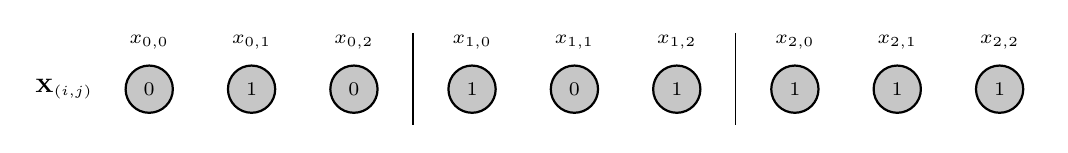
\begin{tikzpicture}[shorten <=1pt,->,draw=black!100]
 	\scriptsize
 	\tikzstyle{label}=[text width=3em, text centered]
 	\tikzstyle{annot}=[text width=2.5em]
 	\tikzstyle{d-node}=[circle,draw=black!100,fill=gray!45,thick,inner sep=2pt,minimum size=6mm]
	
 	\def \china{0.6cm}
 	\def \data{0cm}
	
 	\node[annot] (d-layer) at (0cm,\data) {$\mathbf{X}_{(i,j)}$};
 	\draw[-] (4.45cm, \china+1.5mm) -- (4.45cm, \data-4.5mm);
 	\draw[-] (8.55cm, \china+1.5mm) -- (8.55cm, \data-4.5mm);
 	%\draw[-] (-1cm, \china+.5cm) -- (13cm, \china+.5cm);
 	%\draw[-] (-1cm, \data-.5cm) -- (13cm, \data-.5cm);
	
 	\node[label] 	(dl00)	at (1.1cm,\china)		{$x_{0,0}$};
 	\node[label] 	(dl01)	at (2.4cm,\china)		{$x_{0,1}$};
 	\node[label] 	(dl02)	at (3.7cm,\china)	 	{$x_{0,2}$};
	
 	\node[label] 	(dl10)	at (5.2cm,\china) 		{$x_{1,0}$};
 	\node[label] 	(dl11) 	at (6.5cm,\china)   	{$x_{1,1}$};
 	\node[label] 	(dl12)	at (7.8cm,\china)		{$x_{1,2}$};
	
 	\node[label] 	(dl20) 	at (9.3cm,\china)  		{$x_{2,0}$};
 	\node[label] 	(dl21)	at (10.6cm,\china) 		{$x_{2,1}$};
 	\node[label] 	(dl22) 	at (11.9cm,\china)   	{$x_{2,2}$};
	
 	\node[d-node] 	(d00)	at (1.1cm,\data)		{$0$};
 	\node[d-node] 	(d01)	at (2.4cm,\data)		{$1$};
 	\node[d-node] 	(d02)	at (3.7cm,\data)		{$0$};

 	\node[d-node] 	(d10)	at (5.2cm,\data)		{$1$};
 	\node[d-node] 	(d11)	at (6.5cm,\data)		{$0$};
 	\node[d-node] 	(d12)	at (7.8cm,\data)		{$1$};
	
 	\node[d-node] 	(d20)	at (9.3cm,\data)		{$1$};
 	\node[d-node] 	(d21)	at (10.6cm,\data)		{$1$};
 	\node[d-node] 	(d22)	at (11.9cm,\data)		{$1$};
 \end{tikzpicture}
 %\label{fig:example:subfig0-1}
 }
 \end{center}

 \usetikzlibrary{positioning}
 %\begin{minipage}{.3\textwidth}
 \begin{center}
 \subfigure[Learning in Progress\label{fig:example:subfig1-1}]{
 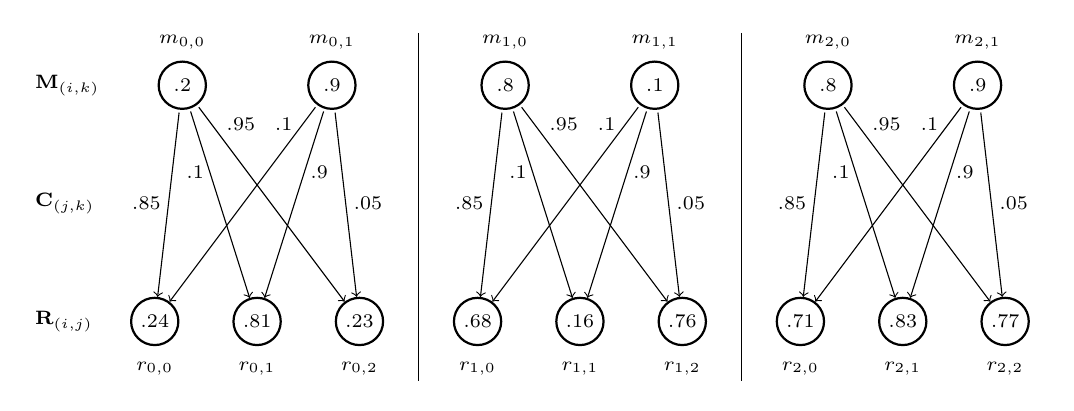
\begin{tikzpicture}[shorten <=1pt,->,draw=black!100]
 	\footnotesize
 	\def \attic{5.95cm}
 	\def \rowtwoht{5.4cm}
 	\def \weightlevel{3.9cm}
 	\def \rowoneht{2.4cm}
 	\def \basement{1.8cm}
% 	\def \data{1cm}
% 	\def \china{0cm}
	
 	\tikzstyle{m-node}=[circle,draw=black!100,thick,inner sep=2pt,minimum size=6mm]
 	\tikzstyle{r-node}=[circle,draw=black!100,thick,inner sep=2pt,minimum size=6mm]
 	\tikzstyle{d-node}=[circle,draw=black!100,fill=gray!45,thick,inner sep=2pt,minimum size=6mm]
 	%\tikzstyle{dots}=[text width=5ex, text centered]
 	\tikzstyle{annot}=[text width=3em]
 	% labels
 	\tikzstyle{label}=[text width=3em, text centered]
 	\tikzstyle{formula}=[text width=30em, text centered]
	
 	\scriptsize
 	\node[annot] (hidden-layer) at (0cm,\rowtwoht) {$\mathbf{M}_{(i,k)}$};
 	\node[annot] (weights) at (0cm,\weightlevel) {$\mathbf{C}_{(j,k)}$};
 	\node[annot] (r-layer) at (0cm,\rowoneht) {$\mathbf{R}_{(i,j)}$};
	
 	% hidden layer
 	\scriptsize
 	\node[m-node] 	(m00)	at (1.45cm,\rowtwoht)		{$.2$};
 	\node[m-node] 	(m01)	at (3.35cm,\rowtwoht)		{$.9$};
 	\node[m-node] 	(m10)	at (5.55cm,\rowtwoht) 	{$.8$};
 	\node[m-node] 	(m11)	at (7.45cm,\rowtwoht)	 	{$.1$};
 	\node[m-node] 	(m20)	at (9.65cm,\rowtwoht) 	{$.8$};
 	\node[m-node] 	(m21)	at (11.55cm,\rowtwoht)	 	{$.9$};
	
 	%\footnotesize
 	\node[label]	(ml00) 	at (1.45cm,\attic)		{$m_{0,0}$}; %1.75 -> 1.45
 	\node[label]	(ml01) 	at (3.35cm,\attic)		{$m_{0,1}$}; %3.05 -> 3.35
 	\node[label] 	(ml10)	at (5.55cm,\attic) 	{$m_{1,0}$};     %5.85 -> 5.55
 	\node[label] 	(ml11)	at (7.45cm,\attic)	 	{$m_{1,1}$}; %7.15 -> 7.45
 	\node[label] 	(ml20)	at (9.65cm,\attic) 	{$m_{2,0}$};     %9.95 -> 9.65
 	\node[label] 	(ml21)	at (11.55cm,\attic)	 	{$m_{2,1}$}; %11.25 -> 11.55
	
 	\scriptsize
 	\node[r-node] 	(r00)	at (1.1cm,\rowoneht)		{$.24$};
 	\node[r-node] 	(r01)	at (2.4cm,\rowoneht)		{$.81$};
 	\node[r-node] 	(r02)	at (3.7cm,\rowoneht)	 	{$.23$};
	
 	\node[r-node] 	(r10)	at (5.2cm,\rowoneht) 		{$.68$};
 	\node[r-node] 	(r11) 	at (6.5cm,\rowoneht)   	{$.16$};
 	\node[r-node] 	(r12)	at (7.8cm,\rowoneht)		{$.76$};
	
 	\node[r-node] 	(r20) 	at (9.3cm,\rowoneht)  		{$.71$};
 	\node[r-node] 	(r21)	at (10.6cm,\rowoneht) 		{$.83$};
 	\node[r-node] 	(r22) 	at (11.9cm,\rowoneht)   	{$.77$};
	
 	\node[label] 	(rl00)	at (1.1cm,\basement)		{$r_{0,0}$};
 	\node[label] 	(rl01)	at (2.4cm,\basement)		{$r_{0,1}$};
 	\node[label] 	(rl02)	at (3.7cm,\basement)	 	{$r_{0,2}$};
	
 	\node[label] 	(rl10)	at (5.2cm,\basement) 		{$r_{1,0}$};
 	\node[label] 	(rl11) 	at (6.5cm,\basement)   	{$r_{1,1}$};
 	\node[label] 	(rl12)	at (7.8cm,\basement)		{$r_{1,2}$};
	
 	\node[label] 	(rl20) 	at (9.3cm,\basement)  		{$r_{2,0}$};
 	\node[label] 	(rl21)	at (10.6cm,\basement) 		{$r_{2,1}$};
 	\node[label] 	(rl22) 	at (11.9cm,\basement)   	{$r_{2,2}$};

 	\draw[-] (4.45cm, \attic+1.5mm) -- (4.45cm, \basement-1.5mm);
 	\draw[-] (8.55cm, \attic+1.5mm) -- (8.55cm, \basement-1.5mm);

 	\scriptsize
 	\path
 		(m00)	edge	node [left] 	{$.85$}	(r00)
 		(m00)	edge	node [left,xshift=-1mm,yshift=4mm]	{$.1$}	(r01)
 		(m00)	edge	node [left,xshift=-1mm,yshift=10mm]	{$.95$}	(r02)

 		(m01)	edge	node [right,xshift=3mm,yshift=10mm]	{$.1$}	(r00)
 		(m01)	edge	node [right,xshift=1mm,yshift=4mm]	{$.9$}	(r01)
 		(m01)	edge	node [right]	{$.05$}	(r02)
 		%
 		(m10)	edge	node [left] 	{$.85$}	(r10)
 		(m10)	edge	node [left,xshift=-1mm,yshift=4mm]	{$.1$}	(r11)
 		(m10)	edge	node [left,xshift=-1mm,yshift=10mm] {$.95$}	(r12)
		
 		(m11)	edge	node [right,xshift=3mm,yshift=10mm]	{$.1$}	(r10)
 		(m11)	edge	node [right,xshift=1mm,yshift=4mm]	{$.9$}	(r11)
 		(m11)	edge	node [right]	{$.05$}	(r12)
 		%
 		(m20)	edge	node [left]	{$.85$}	(r20)
 		(m20)	edge	node [left,xshift=-1mm,yshift=4mm]	{$.1$}	(r21)
 		(m20)	edge	node [left,xshift=-1mm,yshift=10mm]	{$.95$} (r22)
		
 		(m21)	edge	node [right,xshift=3mm,yshift=10mm]		{$.1$}	(r20)
 		(m21)	edge	node [right,xshift=1mm,yshift=4mm]{$.9$}	(r21)
 		(m21)	edge	node [right]	{$.05$}	(r22);		
		
 \end{tikzpicture}
 %\label{fig:example:subfig1-1}
 }
 \subfigure[Convergence\label{fig:example:subfig2-1}]{

 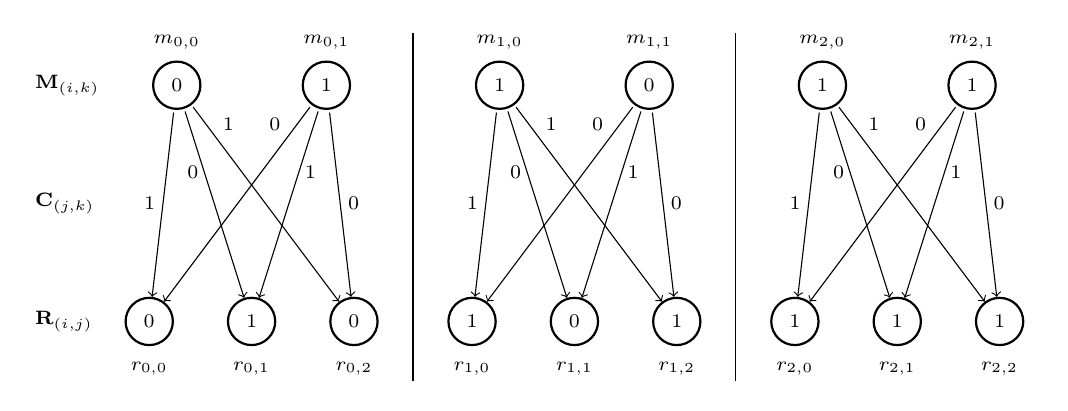
\begin{tikzpicture}[shorten <=1pt,->,draw=black!100]
 	\footnotesize
 	\def \attic{5.95cm}
 	\def \rowtwoht{5.4cm}
 	\def \weightlevel{3.9cm}
 	\def \rowoneht{2.4cm}
 	\def \basement{1.8cm}
% 	\def \data{1cm}
% 	\def \china{0cm}
	
 	\scriptsize
 	\tikzstyle{m-node}=[circle,draw=black!100,thick,inner sep=2pt,minimum size=6mm]
 	\tikzstyle{r-node}=[circle,draw=black!100,thick,inner sep=2pt,minimum size=6mm]
 	\tikzstyle{d-node}=[circle,draw=black!100,fill=gray!45,thick,inner sep=2pt,minimum size=6mm]
 	\tikzstyle{annot}=[text width=2.5em]
 	% labels
 	\tikzstyle{label}=[text width=3em, text centered]
 	\tikzstyle{formula}=[text width=30em, text centered]
 	\node[annot] (hidden-layer) at (0cm,\rowtwoht) {$\mathbf{M}_{(i,k)}$};
 	\node[annot] (weights) at (0cm,\weightlevel) {$\mathbf{C}_{(j,k)}$};
 	\node[annot] (r-layer) at (0cm,\rowoneht) {$\mathbf{R}_{(i,j)}$};
	
 	\node[m-node] 	(m00)	at (1.45cm,\rowtwoht)		{$0$};
 	\node[m-node] 	(m01)	at (3.35cm,\rowtwoht)		{$1$};
 	\node[m-node] 	(m10)	at (5.55cm,\rowtwoht) 	{$1$};
 	\node[m-node] 	(m11)	at (7.45cm,\rowtwoht)	 	{$0$};
 	\node[m-node] 	(m20)	at (9.65cm,\rowtwoht) 	{$1$};
 	\node[m-node] 	(m21)	at (11.55cm,\rowtwoht)	 	{$1$};
	
 	\node[label]	(ml00) 	at (1.45cm,\attic)		{$m_{0,0}$};
 	\node[label]	(ml01) 	at (3.35cm,\attic)		{$m_{0,1}$};
 	\node[label] 	(ml10)	at (5.55cm,\attic) 	{$m_{1,0}$};
 	\node[label] 	(ml11)	at (7.45cm,\attic)	 	{$m_{1,1}$};
 	\node[label] 	(ml20)	at (9.65cm,\attic) 	{$m_{2,0}$};
 	\node[label] 	(ml21)	at (11.55cm,\attic)	 	{$m_{2,1}$};
	
 	\node[r-node] 	(r00)	at (1.1cm,\rowoneht)		{$0$};
 	\node[label] 	(rl00)	at (1.1cm,\basement)		{$r_{0,0}$};
 	\node[r-node] 	(r01)	at (2.4cm,\rowoneht)		{$1$};
 	\node[label] 	(rl01)	at (2.4cm,\basement)		{$r_{0,1}$};
 	\node[r-node] 	(r02)	at (3.7cm,\rowoneht)	 	{$0$};
 	\node[label] 	(rl02)	at (3.7cm,\basement)	 	{$r_{0,2}$};
	
 	\node[r-node] 	(r10)	at (5.2cm,\rowoneht) 		{$1$};
 	\node[label] 	(rl10)	at (5.2cm,\basement) 		{$r_{1,0}$};
 	\node[r-node] 	(r11) 	at (6.5cm,\rowoneht)   		{$0$};
 	\node[label] 	(rl11) 	at (6.5cm,\basement)   		{$r_{1,1}$};
 	\node[r-node] 	(r12)	at (7.8cm,\rowoneht)		{$1$};
 	\node[label] 	(rl12)	at (7.8cm,\basement)		{$r_{1,2}$};
	
 	\node[r-node] 	(r20) 	at (9.3cm,\rowoneht)  		{$1$};
 	\node[label] 	(rl20) 	at (9.3cm,\basement)  		{$r_{2,0}$};
 	\node[r-node] 	(r21)	at (10.6cm,\rowoneht) 		{$1$};
 	\node[label] 	(rl21)	at (10.6cm,\basement) 		{$r_{2,1}$};
 	\node[r-node] 	(r22) 	at (11.9cm,\rowoneht)   		{$1$};
 	\node[label] 	(rl22) 	at (11.9cm,\basement)   		{$r_{2,2}$};
	
 	\draw[-] (4.45cm, \attic+1.5mm) -- (4.45cm, \basement-1.5mm);
 	\draw[-] (8.55cm, \attic+1.5mm) -- (8.55cm, \basement-1.5mm);

 	\path
 		(m00)	edge	node [left] 	{$1$}	(r00)
 		(m00)	edge	node [left,xshift=-1mm,yshift=4mm]	{$0$}	(r01)
 		(m00)	edge	node [left,xshift=-3mm,yshift=10mm]	{$1$}	(r02)

 		(m01)	edge	node [right,xshift=3mm,yshift=10mm]	{$0$}	(r00)
 		(m01)	edge	node [right,xshift=1mm,yshift=4mm]	{$1$}	(r01)
 		(m01)	edge	node [right]	{$0$}	(r02)
 		%
 		(m10)	edge	node [left] 	{$1$}	(r10)
 		(m10)	edge	node [left,xshift=-1mm,yshift=4mm]	{$0$}	(r11)
 		(m10)	edge	node [left,xshift=-3mm,yshift=10mm] {$1$}	(r12)
		
 		(m11)	edge	node [right,xshift=3mm,yshift=10mm]	{$0$}	(r10)
 		(m11)	edge	node [right,xshift=1mm,yshift=4mm]	{$1$}	(r11)
 		(m11)	edge	node [right]	{$0$}	(r12)
 		%
 		(m20)	edge	node [left]	{$1$}	(r20)
 		(m20)	edge	node [left,xshift=-1mm,yshift=4mm]	{$0$}	(r21)
 		(m20)	edge	node [left,xshift=-3mm,yshift=10mm]	{$1$} (r22)
		
 		(m21)	edge	node [right,xshift=3mm,yshift=10mm]		{$0$}	(r20)
 		(m21)	edge	node [right,xshift=1mm,yshift=4mm]{$1$}	(r21)
 		(m21)	edge	node [right]	{$0$}	(r22);		
 \end{tikzpicture}
 %\label{fig:example:subfig2-1}
 }
 \begin{framed}
 	\centering
 	\small
 	where
 	$\begin{aligned}
 	   r_{i,j} = 1 - \Pi_{k=1}^{K} (1 - m_{i,k}c_{j,k}) 
 	\end{aligned}$
 \end{framed}
 \caption{MCMM example showing learning in progress}
 \label{fig:example-1}
 \end{center}
 \end{figure}

Figure~\ref{fig:example-1} shows a simple MCMM at two distinct stages. Figure~\ref{fig:example:subfig1-1} shows the MCMM before convergence, while learning is still in progress. The surface and hidden-unit activities at this stage are still greater than $0$ and less than $1$, though they are on their way to either $0$ or $1$. Figure~\ref{fig:example:subfig2-1}, on the other hand, shows the MCMM after it has converged, when the learning process is complete.

The input data matrix for the MCMM in figure~\ref{fig:example-1} consists of three data points (i.e., $I = 3$).
The hidden cluster activities $\mathbf{M}$, the weights $\mathbf{C}$, the surface-unit vectors $\mathbf{R}$,
and the mixing function together constitute a model that reproduces the
observed data points $\mathbf{X}$.
The $K = 2$ nodes in each $\mathbf{m}_i$
%_{i,k}$ 
are the hidden units and represent cluster-membership activities. There are three cluster-membership vectors $m_{i}$, one for each $i \in I$, i.e., one for each data point. Because there are two clusters, each cluster-membership vector has two components. For instance, $\textbf{m}_{0} = [0, 1]$, which means the first data point $\textbf{x}_{0}$ does not belong to the first cluster, but \emph{does} belong to the second. By contrast, $\textbf{m}_{1} = [1,0]$ indicates that $\textbf{x}_{1}$ belongs to the first cluster, but not to the second. Finally, $\textbf{m}_{2} = [1,1]$ indicates that  $\textbf{x}_{2}$ belongs to \emph{both} clusters. 

These cluster-membership vectors make more sense when we consider them in light of this 
MCMM's $J \times K$ ($3 \times 2$) $\textbf{C}$ matrix, namely, %The two %(transposed) 
%column-vectors
% \begin{align}
%        \textbf{C}  &= \begin{bmatrix}
%          c_{0,0} = 0 \quad c_{0,1}= 1 \\
%           c_{1,0} = 1 \quad c_{1,1} = 0 \\
%           c_{2,0} = 0 \quad c_{2,1} = 1 \\
%         \end{bmatrix} \hspace{12pt}
\begin{equation*}
        \textbf{C}  = \begin{bmatrix}
          0 \quad 1 \\
           1 \quad 0 \\
           0 \quad 1 \\
         \end{bmatrix} \hspace{12pt},
 \end{equation*}
%        \textbf{C}^{\textsf{T}} &= \begin{bmatrix} \\
%          c_{0,0} = 0 \quad c_{0,1} = 1  \quad  c_{0,2} = 0 \\
%           c_{1,0}=1 \quad c_{1,1}= 0  \quad  c_{1,2} = 1
%         \end{bmatrix}
whose two columns are the centroids of the two clusters. %That is, the column %that is, the column vector  
%\begin{equation*}
%%\textbf{c}^{\textsf{T}}_{k=0}   =
%\textbf{C}[\cdot,0] =
% %\begin{bmatrix}$c_{2,0}$ \quad $c_{1,0}$  \quad  $c_{0,0}$\end{bmatrix}
%%\textbf{c}^{\textsf{T}}_{0}  &= 
%\begin{bmatrix}
%          0 \\
%           1 \\
%          0 \\
%         \end{bmatrix} 
% \end{equation*}
%is the centroid of the cluster with index $k = 0$, and
%\begin{equation*}
% %\textbf{c}^{\textsf{T}}_{k=1}   =
% \textbf{C}[\cdot,1] =
% %\begin{bmatrix}$c_{2,0}$ \quad $c_{1,0}$  \quad  $c_{0,0}$\end{bmatrix}
%%\textbf{c}^{\textsf{T}}_{0}  &= 
%\begin{bmatrix}
%         1 \\
%           0 \\
%          1 
%         \end{bmatrix}
%\end{equation*}
%is the centroid of the cluster with index $k = 1$.
%We can transpose these two column vectors to express them as row vectors:
%\begin{align*}
%\mathbf{C}^{\textsf{T}}[0,\cdot]  \,\, &= \,\, \mathbf{c}^{\textsf{T}}_{0} \,\, = \,\,  [\,0 \,\, 1 \,\,  0 \, ] \qquad \text{centroid of cluster $k = 0$}\\
%\mathbf{C}^{\textsf{T}}[1,\cdot]\,\, &= \,\,  \mathbf{c}^{\textsf{T}}_{1} \,\, = \,\, [\,1 \,\, 0 \,\,  1 \, ]
%\qquad \text{centroid of cluster $k = 1$} \\
%\end{align*}
%  is the centroid of the cluster indexed $k=0$
%  \textbf{c}^{\textsf{T}}_{k=1}  &= \begin{bmatrix}
%           x_{1} \\
%           x_{2} \\
%           \vdots \\
%           x_{m}
%         \end{bmatrix}
%  \end{align}
%$\textbf{C}^\textsf{T}[0,:] = [0,1,0]$ and $\textbf{C}^\textsf{T}[1,:]  = [1,0,1]$ (for $j = 0$ and $j =1$) 
%$\textbf{C}[\bullet,0] = [0,1,0]$ (for $k = 0$ and $j \in \{ 0,1,2\}$) and $\textbf{C}[\bullet,1]  = [1,0,1]$ (for $k = 1$ and $j \in \{ 0,1,2\}$)
%(for $k = 0$ and $k=1$, respectively; the three components in each of vectors correspond to the three $j$ indices) 
%are the \emph{centroids} of the first and second clusters, respectively. 
A cluster's centroid is essentially a sort of average or composite of its member vectors; it represents the feature values that its members have in common and thus concisely represents the cluster's meaning, i.e., what it is that makes the cluster an equivalence class. % thus serve as a label for the cluster in question.

In our example, the first data point $\textbf{x}_0 = [0,1,0]$ is clearly a member of cluster 0, as it is identical to the centroid of cluster 0; no other cluster is necessary to account its components. %$[0,1,0]$. 
Similarly, the second data point $\textbf{x}_1 = [1,0,1]$ is a member of cluster $1$, as it is identical to cluster $1$'s centroid $[1,0,1]$; no other cluster is necessary to explain its components. %all of its components are explained by cluster $1$.
%Again, the data point is identical to the centroid, so cluster 1 is sufficient to account for the components of  $\textbf{x}_1$.
However, the third data point $\textbf{x}_2 = [1,1,1]$ cannot be exclusively attributed to either cluster $0$ or cluster $1$; rather, it shows in its components the influence of \emph{both}: The middle $1$ can be attributed to cluster $0$
% it is the $1$ in cluster $0$'s 
(centroid $ [0,1,0]$),
while the first and third $1$s are due to cluster $1$ (centroid $ [1,0,1]$). 
%,  the influence of \emph{both} clusters is evident in the third data point $\textbf{x}_2 = [1,1,1]$; the 
Table~\ref{tab:cl-members} shows the members as well as the centroids of each of the two clusters: Notice that the active components in each cluster centroid correspond to the shared component values among the cluster's members.

 \begin{table}[!h]
\begin{mdframed}
\centering
\setlength{\extrarowheight}{8pt}
\begin{tabular}{ccc}
\toprule
Cluster index ($k$) & Member Data Points & Cluster Centroid \\ \midrule
 $0$ &  $[0,\mathbf{1},0]$, $[1,\mathbf{1},1]$ & $[0,1,0]$\\ 
 $1$  & $[\mathbf{1},0,\mathbf{1}]$, $[\mathbf{1},1,\mathbf{1}]$ & $[1,0,1]$\\
 \bottomrule
 \end{tabular}
\caption{\emph{Clusters from Figure~\ref{fig:example-1} and their Centroids.} The active features in each cluster's centroid are the \emph{shared} active features among the cluster's members.}
\label{tab:cl-members}
\end{mdframed}
\end{table}

%Figure~\ref{fig:example:subfig1-1} shows the MCMM when it is in the process of learning. %We can see that while learning is in 
%As it is learning, i.e., as it is reducing its reconstruction error, the cluster-membership indicators in $\mathbf{M}$ are in flux, as are the components of 
%cluster centroids in $\textbf{C}$ (also known as the weights). As learning progresses, each value in $\mathbf{M}$ and  $\textbf{C}$ gradually approaches either 0 or 1. At convergence, the reconstruction vectors match the original data points, and all activities in $\mathbf{M}$ and $\textbf{C}$ are either $0$ or $1$, as in figure~\ref{fig:example:subfig2-1}.

% they converge to values of 0 and
%1.  At convergence, a reconstruction node $r_{i,j}$ is 1 if at least one
%$m_{i,k}c_{j,k} = 1$ (and $0$ otherwise).

\section{Conclusion}
This chapter has been the culminating chapter of what can be regarded as 
Part 1 of this thesis. These first four chapters have been concerned with 
linking autosegmental morphological theory to an unsupervised learning 
algorithm, in particular, the MCMM. It has advanced the hypothesis 
(first introduced as proposition~\ref{prop:nlns} in chapter~\ref{ch:intro}) 
that a ULM algorithm/system can learn nonconcatenative morphology if it 
is nonlinear and nonsequential. We have seen that MCMMs meet these criteria. 
We will now adjust our course somewhat as we begin the thesis’s second part, 
which will be concerned with the actual testing of the first part’s hypothesis.
 This testing has taken the form of building Multimorph, 
 an MCMM-driven system 
 %(as we have established the MCMM’s nonlinearity 
% and nonsequentiality in this chapter and chapter~\ref{ch:graph} preceding chapters) 
 and testing it on Hebrew words, which contain plenty of nonconcatenative morphology. 
Additional research questions were raised along the way, and we 
 will address these in the following chapters. The next chapter discusses the 
 targets of Multimorph's learning, that is, the type of categories one should 
 look for in its output. This is a crucial question for purposes of evaluation.
